%%%%%%%%%%%%%%%%%%%%%%%%%%%%%%%%%%%%%%%%%%%%%%%%%%%%%%%%%%%%%%%%%%%%%
%% This is a (brief) model paper using the achemso class
%% The document class accepts keyval options, which should include
%% the target journal and optionally the manuscript type.
%%%%%%%%%%%%%%%%%%%%%%%%%%%%%%%%%%%%%%%%%%%%%%%%%%%%%%%%%%%%%%%%%%%%%
\documentclass[journal=jctc,manuscript=article]{achemso}

%%%%%%%%%%%%%%%%%%%%%%%%%%%%%%%%%%%%%%%%%%%%%%%%%%%%%%%%%%%%%%%%%%%%%
%% Place any additional packages needed here.  Only include packages
%% which are essential, to avoid problems later. Do NOT use any
%% packages which require e-TeX (for example etoolbox): the e-TeX
%% extensions are not currently available on the ACS conversion
%% servers.
%%%%%%%%%%%%%%%%%%%%%%%%%%%%%%%%%%%%%%%%%%%%%%%%%%%%%%%%%%%%%%%%%%%%%
\usepackage[version=3]{mhchem} % Formula subscripts using \ce{}

\usepackage{color}
\usepackage{graphicx}
\usepackage{mhchem}
\usepackage{physics}
\usepackage{subcaption}

\usepackage[utf8]{inputenc}
\usepackage[T1]{fontenc}

\usepackage[capitalise]{cleveref}  % Need to load after amsmath.
%%%%%%%%%%%%%%%%%%%%%%%%%%%%%%%%%%%%%%%%%%%%%%%%%%%%%%%%%%%%%%%%%%%%%
%% If issues arise when submitting your manuscript, you may want to
%% un-comment the next line.  This provides information on the
%% version of every file you have used.
%%%%%%%%%%%%%%%%%%%%%%%%%%%%%%%%%%%%%%%%%%%%%%%%%%%%%%%%%%%%%%%%%%%%%
%%\listfiles

%%%%%%%%%%%%%%%%%%%%%%%%%%%%%%%%%%%%%%%%%%%%%%%%%%%%%%%%%%%%%%%%%%%%%
%% Place any additional macros here.  Please use \newcommand* where
%% possible, and avoid layout-changing macros (which are not used
%% when typesetting).
%%%%%%%%%%%%%%%%%%%%%%%%%%%%%%%%%%%%%%%%%%%%%%%%%%%%%%%%%%%%%%%%%%%%%
\newcommand*\mycommand[1]{\texttt{\emph{#1}}}

\graphicspath{{toc/}{figures/}}

%%%%%%%%%%%%%%%%%%%%%%%%%%%%%%%%%%%%%%%%%%%%%%%%%%%%%%%%%%%%%%%%%%%%%
%% Meta-data block
%% ---------------
%% Each author should be given as a separate \author command.
%%
%% Corresponding authors should have an e-mail given after the author
%% name as an \email command. Phone and fax numbers can be given
%% using \phone and \fax, respectively; this information is optional.
%%
%% The affiliation of authors is given after the authors; each
%% \affiliation command applies to all preceding authors not already
%% assigned an affiliation.
%%
%% The affiliation takes an option argument for the short name.  This
%% will typically be something like "University of Somewhere".
%%
%% The \altaffiliation macro should be used for new address, etc.
%% On the other hand, \alsoaffiliation is used on a per author basis
%% when authors are associated with multiple institutions.
%%%%%%%%%%%%%%%%%%%%%%%%%%%%%%%%%%%%%%%%%%%%%%%%%%%%%%%%%%%%%%%%%%%%%
\author{Laurent Lemmens}
\author{Xeno De Vriendt}
\author{Patrick Bultinck}
\email{Patrick.Bultinck@UGent.be}
\author{Guillaume Acke}
\affiliation{Ghent University, Department of Chemistry - Ghent Quantum Chemistry Group, Krijgslaan 281 (S3), B-9000 Ghent, Belgium}



%%%%%%%%%%%%%%%%%%%%%%%%%%%%%%%%%%%%%%%%%%%%%%%%%%%%%%%%%%%%%%%%%%%%%
%% The document title should be given as usual. Some journals require
%% a running title from the author: this should be supplied as an
%% optional argument to \title.
%%%%%%%%%%%%%%%%%%%%%%%%%%%%%%%%%%%%%%%%%%%%%%%%%%%%%%%%%%%%%%%%%%%%%
\title{Analyzing the behavior of spin phases in external magnetic fields by means of spin constrained states}

%%%%%%%%%%%%%%%%%%%%%%%%%%%%%%%%%%%%%%%%%%%%%%%%%%%%%%%%%%%%%%%%%%%%%
%% Some journals require a list of abbreviations or keywords to be
%% supplied. These should be set up here, and will be printed after
%% the title and author information, if needed.
%%%%%%%%%%%%%%%%%%%%%%%%%%%%%%%%%%%%%%%%%%%%%%%%%%%%%%%%%%%%%%%%%%%%%
% \abbreviations{IR,NMR,UV}
% \keywords{American Chemical Society, \LaTeX}

%%%%%%%%%%%%%%%%%%%%%%%%%%%%%%%%%%%%%%%%%%%%%%%%%%%%%%%%%%%%%%%%%%%%%
%% The manuscript does not need to include \maketitle, which is
%% executed automatically.
%%%%%%%%%%%%%%%%%%%%%%%%%%%%%%%%%%%%%%%%%%%%%%%%%%%%%%%%%%%%%%%%%%%%%
\begin{document}

%%%%%%%%%%%%%%%%%%%%%%%%%%%%%%%%%%%%%%%%%%%%%%%%%%%%%%%%%%%%%%%%%%%%%
%% The "tocentry" environment can be used to create an entry for the
%% graphical table of contents. It is given here as some journals
%% require that it is printed as part of the abstract page. It will
%% be automatically moved as appropriate.
%%%%%%%%%%%%%%%%%%%%%%%%%%%%%%%%%%%%%%%%%%%%%%%%%%%%%%%%%%%%%%%%%%%%%
\begin{tocentry}

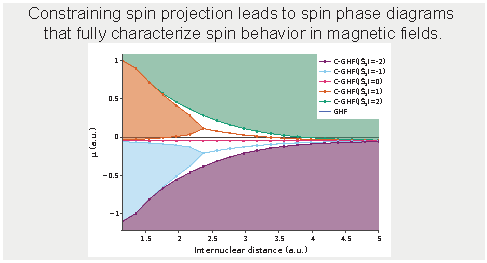
\includegraphics{graphical-TOC}

\end{tocentry}

%%%%%%%%%%%%%%%%%%%%%%%%%%%%%%%%%%%%%%%%%%%%%%%%%%%%%%%%%%%%%%%%%%%%%
%% The abstract environment will automatically gobble the contents
%% if an abstract is not used by the target journal.
%%%%%%%%%%%%%%%%%%%%%%%%%%%%%%%%%%%%%%%%%%%%%%%%%%%%%%%%%%%%%%%%%%%%%
\begin{abstract}
    During molecular dissociation in the presence of an external uniform magnetic field, electrons flip their spin anti-parallel to the magnetic field due to the stabilizing influence of the spin Zeeman operator.
    Although generalized Hartree-Fock descriptions furnish the optimal mean-field energetic description of such bond breaking processes, they are allowed to break $\hat{S}_z$-symmetry leading to intricate and unexpected spin phases and phase transitions.
    In this work, we show that the behavior of these molecular spin phases can be interpreted in terms of spin phase diagrams constructed by constraining states to target expectation values of projected spin.
    The underlying constrained states offer a complete electronic characterization of spin phases and spin phase transitions as they can be analyzed using standard quantum chemical tools.
    As the constrained states effectively span the entire phase space, they could provide an excellent starting point for post-Hartree Fock methods aimed at gaining more electron correlation or regaining spin symmetry.
\end{abstract}

%%%%%%%%%%%%%%%%%%%%%%%%%%%%%%%%%%%%%%%%%%%%%%%%%%%%%%%%%%%%%%%%%%%%%
%% Start the main part of the manuscript here.
%%%%%%%%%%%%%%%%%%%%%%%%%%%%%%%%%%%%%%%%%%%%%%%%%%%%%%%%%%%%%%%%%%%%%
\section{Introduction}
    When subjected to external magnetic fields, molecular systems display exotic chemistry because of competing magnetic and Coulomb interactions \cite{Schmelcher.1989, Schmelcher.1997, Lange.2012, Schmelcher.2012}. Attempts to accurately describe the effects of these competing forces have sparked recent advances in mean-field \cite{Tellgren.2008, Tellgren.2013, Boblest.2014, Reynolds.2014, Sen.2018, Sen.2018a, Sen.2019, Sun.2019, Lehtola.2019, Bischoff.2020}, configuration interaction \cite{Lange.2012, Reynolds.2018, Austad.2020}, coupled cluster \cite{Stopkowicz.2015, Stopkowicz.2018, Hampe.2017, Hampe.2019, Hampe.2020, Thomas.2021} and density functional theories \cite{Sagvolden.2013, Tellgren.2014, Furness.2015, Reimann.2015, Furness.2016, Reimann.2017, Reimann.2018, Laestadius.2019, Irons.2020, Sen.2021, Irons.2021a, Laestadius.2021, Kvaal.2021}, molecular integral evaluation \cite{Tellgren.2008, Tellgren.2012, Irons.2017, Sun.2019, Pausch.2020, Blaschke.2021} and software implementations \cite{LONDON, QCUMBRE, QUEST, Shiozaki.2018, Al-Saadon.2019, Williams-Young.2020, Matthews.2020}, with applications in atomic and molecular properties \cite{Zarycz.2016, Tellgren.2009, Holzer.2019, Sun.2019a, Stetina.2019, Sun.2020, Pagola.2019, Lazzeretti.2020, Wibowo.2021}, and molecular dynamics.\cite{Culpitt.2021, Peters.2021}
    
    The interplay between magnetic and Coulombic forces leads, among other things, to complicated spin behavior during molecular dissociation in the presence of a uniform magnetic field, as the spin Zeeman operator favors spin-flips by paramagnetically stabilizing electrons that are aligned anti-parallel to the magnetic field. 
    Electronic structure models should thus be able to cover multiple spin sectors to adequately characterize such dissociation processes.
    For spin symmetry-adapted methods, this amounts to separate calculations for different spin multiplicities,\cite{Stopkowicz.2015, Sun.2019} which combined yield a segmented potential energy surface. 
    For spin broken methods (also called non-collinear or generalized methods \cite{Small.2015, Henderson.2018}), spin sectors can be mixed as these methods are formulated in terms of two-component spinors that encompass both $\alpha$- and $\beta$-spin character.
    As such, the generalized Hartree-Fock (GHF) method \cite{Fukutome.1981, Lowdin.1992, Hammes-Schiffer.1993, Mayer.1993, Jimenez-Hoyos.2011, Jake.2018, Sen.2018, Sun.2019} leads to smooth potential energy surfaces during molecular dissociation in the presence of external magnetic fields.
    However, as a typical case of Löwdin's symmetry dilemma \cite{Lykos.1963}, these lowest mean-field solutions come at the cost of good spin quantum numbers.

    \begin{figure}
        \centering
        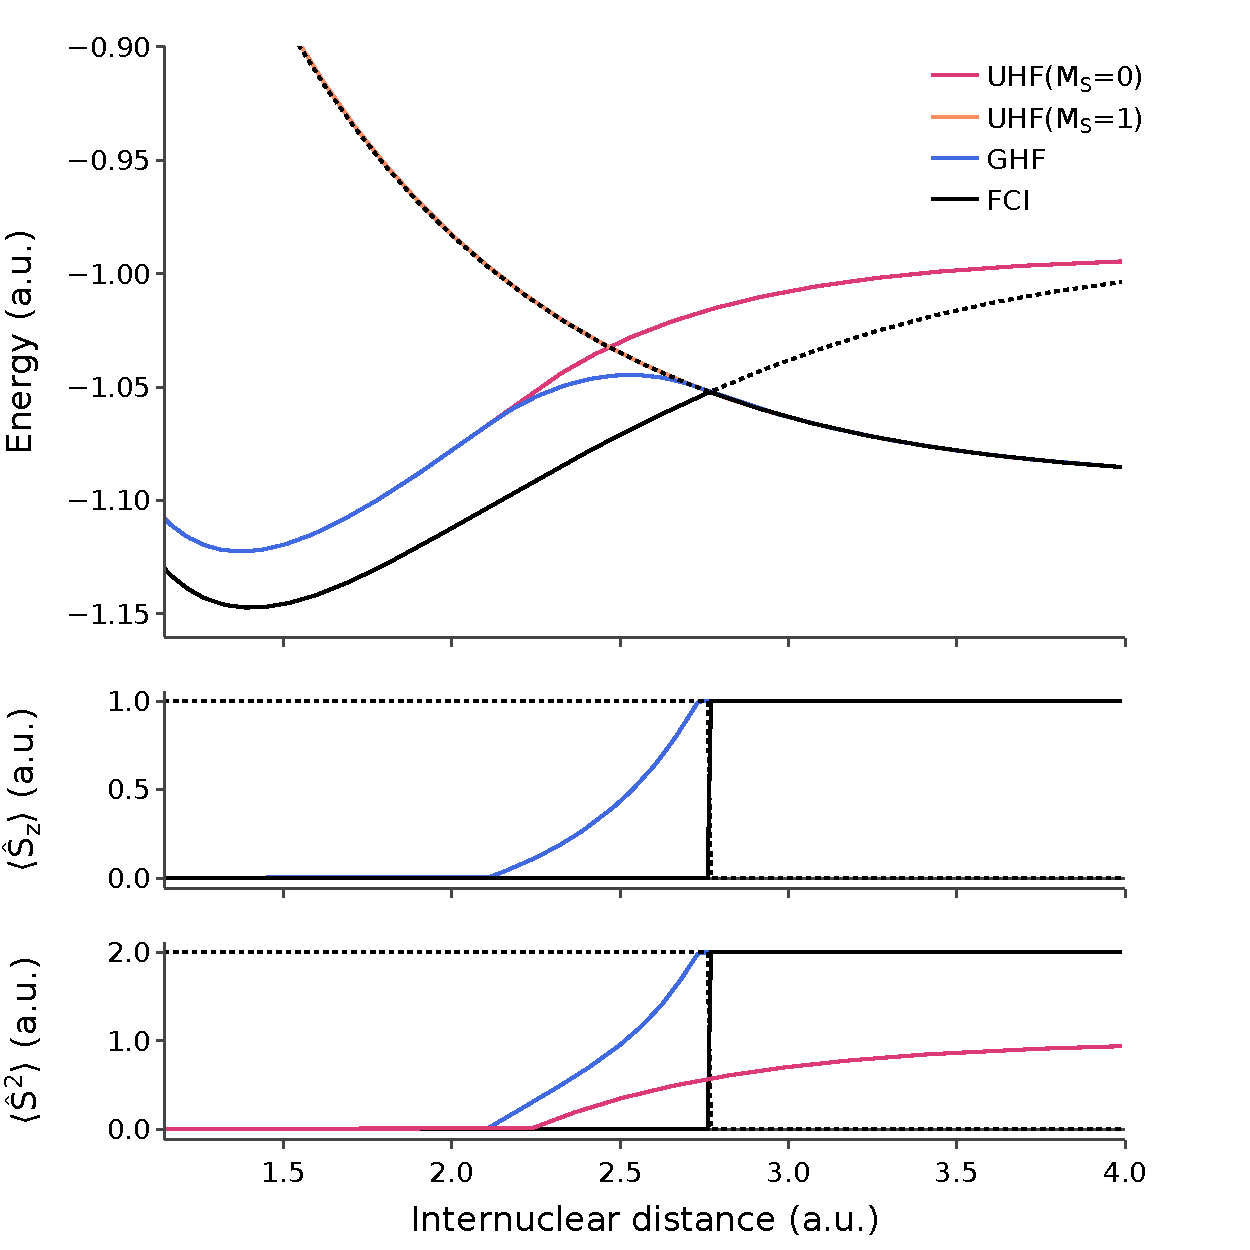
\includegraphics[width=0.65\textwidth]{FCI-vs-U-GHF-E-and-S(H2)}
        \caption{
            Total energy, and $\ev*{\hat{S}_z}$ and $\ev*{\hat{S}^2}$ expectation values for UHF, GHF and FCI during the dissociation of \ce{H2} in the presence of an external uniform magnetic field $\vb{B}_{\text{ext}}=(0,0,-0.1)\text{ a.u}$ where the molecular axis lies on the $x$-axis.
            The UHF calculations are performed for singlet ($M_S=0$) and triplet ($M_S=1$) states.
            The UHF and GHF results for \ce{H2} are discussed by Li and coworkers.\cite{Sun.2019}
            The first excited state for FCI is indicated by the dashed line.
        }
        \label{fig:FCI(with-excited)-vs-U-GHF-E-and-S(H2)}
    \end{figure}

    As first reported by Li and coworkers \cite{Sun.2019}, the GHF description of the dissociation of molecular hydrogen exhibits a gradual increase in $\ev*{\hat{S}_z}$, where the GHF solution transitions between two UHF spin states (cfr. \cref{fig:FCI(with-excited)-vs-U-GHF-E-and-S(H2)}).
    By energetically analyzing the underlying GHF states, Li et al. showed that, at moderate magnetic fields, competing spin exchange and spin Zeeman interactions are tightly balanced, leading to non-integer values for the expectation value of projected spin $\ev*{\hat{S}_z}$ in GHF states \cite{Sun.2019}.
    However, due to this intricately balanced energetic competition, it is very difficult to predict the behavior of $\ev*{\hat{S}_z}$ along the dissociation profiles of other molecular systems and whether $\ev*{\hat{S}_z}$ should always mirror the strictly increasing profile reported for \ce{H2} \cite{Sun.2019}.

    In order to study this spin behavior, we propose to augment the energetic analysis of Li et al. by contrasting the GHF state in question with GHF states where we have \emph{imposed} a target spin expectation value $S_{z, \thinspace \text{target}}$. 
    This allows us to determine what the energetic costs are of only \emph{partially} allowing for certain spin flips and why certain spin sectors are disfavored energetically.
    In order to do so, we extend the theory of Li and coworkers \cite{Sun.2019} with a constrained formalism \cite{Mukherji.1963, Zeiss.1983, Zeiss.1983a, Kaduk.2012, DeVriendt.2021} that allow us to target states with a particular $\ev*{\hat{S}_z}$.
    The resulting formalism allows us to characterize the electronic structure underlying the spin behavior in magnetic fields in terms of the constrained GHF states and \emph{spin phase diagrams} that arise from the associated Lagrange multipliers.
    We show that these spin phase diagrams offer a dual and enriched view on the observed spin behavior during the dissociation of $\ce{H2}$ and equilateral cyclic \ce{H4}.

\section{Theory}

    In this section, we introduce the theoretical framework needed to describe constrained states in external magnetic fields. 
    First, we focus on the one-electron interactions present in such systems and describe the formalism of second quantization with two-components spinors, which allows us to discuss the generalized Hartree-Fock method and its stability conditions. 
    Next, we establish the second-quantized representation of the molecular magnetic Hamiltonian in a generalized spinor basis.
    Finally, we show how the formalism of constraints can be used to constrain states to a given $S_z$.

    \subsection{The one-electron Pauli Hamiltonian} \label{sec:theory:Pauli-Hamiltonian}

        When an electron is subjected to a time-independent external uniform magnetic field $\vb{B}_{\text{ext}}$, its physical interactions are governed by the one-electron Pauli Hamiltonian.
        In a molecular context, under the Born-Oppenheimer approximation, the Pauli Hamiltonian $\vb{h}$ is given in coordinate representation (indicated by the superscript $c$) by \cite{Bransden.2000, Helgaker.2012, Cohen-Tannoudji.2020.Volume2}
        \begin{equation} \label{eq:Pauli-Hamiltonian}
            \vb{h}^c(\vb{r}, \vb{B}_{\text{ext}}, \vb{G})
            = \qty[
                k^c(\vb{r}, \vb{B}_{\text{ext}},\vb{G})
                - \sum_K
                    \frac{Z_K}{r_K}
            ] \thinspace \vb{I}_2
            + \frac{1}{2}
                \boldsymbol{\sigma} \vdot \vb{B}_{\text{ext}}
            \thinspace ,
        \end{equation}
        with $\vb{I}_2$ the $(2 \times 2)$ identity matrix, $\boldsymbol{\sigma}$ the 3-vector of the Pauli matrices
        \begin{equation}
            \sigma_x =
            \begin{pmatrix} 0 & 1 \\ 1 & 0 \end{pmatrix}
            %
            \qquad
            %
            \sigma_y = \begin{pmatrix} 0 & -i \\ i & 0 \end{pmatrix}
            %
            \qquad
            %
            \sigma_z = \begin{pmatrix} 1 & 0 \\ 0 & -1 \end{pmatrix}
            \label{eq:pauli-matrices}
        \end{equation}
        and $k^c$ the (scalar) kinetic energy operator
        \begin{equation} \label{eq:scalar-kinetic-energy-operator}
            k^c(\vb{r}, \vb{B}_{\text{ext}},\vb{G})
            = - \frac{1}{2} \laplacian
            + \frac{1}{2} \thinspace
                \vb{B}_{\text{ext}} \vdot \vb{L}^c(\vb{G})
            + \frac{1}{8} \qty(
                B^2_{\text{ext}} \thinspace r_G^2
                - \qty[ \vb{B}_{\text{ext}} \cdot \vb{r}_G ]^2
            )
            \thinspace .
        \end{equation}
        Here, $\vb{L}^c(\vb{G}) = -i \vb{r}_G \cross \grad$ is the angular momentum operator about the gauge origin $\vb{G}$ of the magnetic vector potential
        \begin{equation} \label{eq:vector-potential}
            \vb{A}_{\text{ext}}(\vb{r})
            = \frac{1}{2} \thinspace
                \vb{B}_{\text{ext}} \cross \vb{r}_G
            \thinspace ,
        \end{equation}
        where we have introduced the short-hand notation $\vb{r}_G = \vb{r} - \vb{G}$.
        The summation in \cref{eq:Pauli-Hamiltonian} is over all nuclei $K$ with charge $Z_K$ and the relative distance between the electron and the nucleus $K$ is $r_K = \norm{\vb{r}-\vb{R}_K}$, where $\vb{R}_K$ is the position of nucleus $K$.

        The total electron-magnetic field interaction consists of three contributions: the orbital Zeeman operator (the second term in \cref{eq:scalar-kinetic-energy-operator}), the diamagnetic operator (the third term in \cref{eq:scalar-kinetic-energy-operator}) and the spin Zeeman operator (the second term in \cref{eq:Pauli-Hamiltonian}) that expresses the interaction of electron spin with the external magnetic field.
        The orbital Zeeman and spin Zeeman terms are paramagnetic terms, i.e. they are first order in the magnetic field, and the diamagnetic term is quadratic in the magnetic field.

    \subsection{Second quantization with spinors} \label{sec:theory:spinors}
        According to \cref{eq:Pauli-Hamiltonian}, the Pauli Hamiltonian $\vb{h}^c$ is a $(2 \times 2)$ \emph{matrix operator}.
        Accordingly, the state of an electron must be characterized by a two-component wave function, i.e. a \emph{spinor} $\boldsymbol{\phi}_P(\vb{r})$ \cite{Sen.2018, Sun.2019, Cohen-Tannoudji.2020.Volume2, Lemmens.2021}
        \begin{equation} \label{eq:spinor}
            \boldsymbol{\phi}_P(\vb{r})
            =
            \begin{pmatrix}
                \phi_P^\alpha(\vb{r}) \\
                \phi_P^\beta(\vb{r})
            \end{pmatrix}
            \thinspace .
        \end{equation}
        
        The elementary annihilation and creation operators $\hat{a}_P$ and $\hat{a}^\dagger_P$ associated with an orthonormal basis $\qty{ \boldsymbol{\phi}_P(\vb{r}) \thinspace | \thinspace P = 1 \cdots M }$ of $M$ two-component spinors obey the fermion anticommutation relations \cite{Surjan.1989, Helgaker.1991, Helgaker.2000, Helgaker.2012, Cohen-Tannoudji.2020.Volume3}
        \begin{equation}
            \comm*{ \hat{a}_P }{ \hat{a}^\dagger_Q }_+
            = \delta_{PQ}
            \qqtext{and}
            \comm*{ \hat{a}^\dagger_P }{ \hat{a}^\dagger_Q }_+
            = 0
            \thinspace .
        \end{equation}
        As the individual spinors in \cref{eq:spinor} are not necessarily eigenvectors of the Pauli matrix $\sigma_z$, the wave functions constructed with the elementary operators $\hat{a}_P$ and $\hat{a}^\dagger_P$ can be symmetry-broken and are not necessarily eigenvectors of the total projected spin $\hat{S}_z$.
        However, when only one of the components of \emph{each} of the spinors is non-zero, the spinors \emph{are} eigenvectors of $\sigma_z$ (i.e. they are \emph{spin-orbitals}), which leads to considerable simplifications in subsequent second quantized derivations \cite{Lemmens.2021}.

        In the full configuration interaction (FCI) method, the wave function model is expressed as a linear combination of all occupation number vectors (ONVs) in a Fock subspace for $M$ spinors and $N$ electrons:\cite{Helgaker.2000}
        \begin{equation}
            \ket{\text{FCI}(\vb{c})}
            = \sum_{\vb{k}} c_{\vb{k}} \ket{\vb{k}}
            \thinspace ,
        \end{equation}
        in which the individual orbitals that appear in the ONVs $\ket{\vb{k}}$ are general two-component spinors (cfr. \cref{eq:spinor}).
        As such, each individual ONV is \emph{not} necessarily an eigenvector of $\hat{S}_z$, guaranteeing the flexibility (but not the restriction) to describe spin non-collinear configurations.
        In traditional (spin-collinear) FCI, the Hamiltonian is diagonalized in different spin sectors of dimensions $\binom{K}{N_\alpha} \binom{K}{N_\beta}$.
        However, in spin \emph{non}-collinear FCI theory, the Hamiltonian is diagonalized in the full Fock space of dimension $\binom{M}{N}$, with $N = N_\alpha + N_\beta$ the total number of electrons in the system.\cite{Helgaker.2000}
        Provided that the Hamiltonian (in spin-collinear FCI) is diagonalized in every spin sector, the resulting spectrum is equal to the spectrum obtained through the diagonalization of the Hamiltonian (in spin non-collinear FCI) in the full Fock space.
        Even though spin non-collinear FCI can be viewed as an unnecessary luxury (as FCI is spin-adapted by definition), we show in this study that the presence of an external magnetic field can induce unexpected transitions between spin sectors during a dissociation process. 
        This renders it very difficult to establish beforehand which spin sectors should be included in conventional, spin-collinear FCI.

        \subsection{Generalized Hartree-Fock and stability conditions}

        The generalized Hartree-Fock (GHF) wave function model\cite{Fukutome.1981, Lowdin.1992} can be expressed as
        \begin{equation}
            \ket{\text{GHF}}
            = \qty(
                \prod_I \hat{a}^\dagger_I
            ) \ket{\text{vac}}
            \thinspace ,
        \end{equation}
        with $\ket{\text{vac}}$ the true Fock vacuum and where $I$ labels those spinors that are occupied in the GHF single-Slater determinant.

        In practice, each of the spinor components is expanded in a known scalar basis (usually an atomic orbital (AO) basis) of $K$ (with $M=2K$) basis functions $\{ \varphi_{\mu}(\vb{r}) \thinspace | \thinspace \mu = 1 \cdots K \}$:
        \begin{equation}
            \phi_P^\sigma(\vb{r})
            = \sum_\mu \varphi_\mu(\vb{r}) C^{\sigma}_{\mu P}
            \thinspace ,
        \end{equation}
        with $\vb{C}$ the expansion coefficient matrix and where we have used the label $\sigma$ to designate either $\alpha$ or $\beta$.
        Minimization of the GHF energy with respect to the spinor expansion coefficients $\vb{C}$, subject to the constraint that the occupied spinors remain orthonormal, leads to the GHF self-consistent field (SCF) equations
        \begin{equation}
            \vb{F} \vb{C} = \vb{S} \vb{C} \boldsymbol{\epsilon}
        \end{equation}
        formulated in the AO basis.
        Here, the Fock matrix $\vb{F}$ has a $(2 \times 2)$ block matrix spin structure:
        \begin{equation}
            \vb{F}
            = \begin{pmatrix}
                \vb{F}^{\alpha \alpha}
                    & \vb{F}^{\alpha \beta} \\
                \vb{F}^{\beta \alpha}
                    & \vb{F}^{\beta \beta}
            \end{pmatrix}
            \thinspace ,
        \end{equation}
        whose off-diagonal blocks consist of the off-diagonal core Hamiltonian and two-electron exchange contributions.\cite{Sen.2018, Sun.2019}
        As in unrestricted Hartree-Fock (UHF) theory off-diagonal blocks in the coefficient matrix $\vb{C}$ vanish, UHF can only account for the spin Zeeman interaction with a magnetic field applied in the $z$-direction.
        In restricted Hartree-Fock (RHF) theory, additionally, the top-left ($\alpha \alpha$) and bottom-right ($\beta \beta$) blocks in $\vb{C}$ are equal.
        As the RHF expectation values of the electronic spin vector operator vanish, RHF cannot describe spin Zeeman interactions.

        When performing Hartree-Fock calculations, it may happen that the solution obtained is not an energy minimum within its own set of constraints (an internal instability) or there may be a lower energy solution if one breaks some specific symmetry (an external instability). As detailed by Stuber and Paldus \cite{stuber2003a}, strictly negative eigenvalues in the Hartree-Fock Hessian $\vb{M}$
        \begin{equation}
            \vb{M}
            = \begin{pmatrix}
                \vb{A} & \vb{B} \\
                \vb{B^*} & \vb{A^*}
            \end{pmatrix}
        \end{equation}
        indicate an instability, and we can follow the eigenvector $\vb{J}$ corresponding to the lowest negative eigenvalue by exponentiating the mixing matrix $\vb{K}$
        \begin{equation}
            \vb{K}
            = \begin{pmatrix}
                \vb{0} & -\vb{J}^\dagger \\
                \vb{J} & \vb{0}
            \end{pmatrix}
        \end{equation}
        and applying the resulting unitary rotation to the spin expansion coefficients $\vb{C}$
        \begin{equation}
            \vb{C}' = \vb{C} e^{-s\vb{K}}
        \end{equation}
        with $s$ a small step in the direction $\vb{K}$ \cite{Goings.2015}. 
        In contrast to RHF and UHF, where following external instabilities requires breaking symmetries, all instabilities in complex GHF are internal as this method has broken spin, time-reversal and complex conjugation symmetries.

    \subsection{The second-quantized molecular magnetic Hamiltonian} \label{sec:theory-sq-molecular}
        In a complete orbital basis, the choice of gauge origin $\vb{G}$ of the magnetic vector potential in \cref{eq:vector-potential} does not influence the value of calculated properties.
        However, in a truncated orbital basis, this gauge origin independence is no longer assured.\cite{Helgaker.1991}
        In order to resolve this so-called gauge origin problem, the $\alpha$- and $\beta$-components of the spinors are expanded in a scalar basis composed of \emph{London} orbitals: \cite{London.1937, Ditchfield.1972, Helgaker.1991, Helgaker.2012}
        \begin{equation}
            \phi_P^{\sigma}(\vb{r}, \vb{B}_{\text{ext}}, \vb{G})
            = \sum_{\mu}
                \omega_{\mu}(\vb{r}, \vb{B}_{\text{ext}}, \vb{G})
                C_{\mu P}^\sigma
            \thinspace ,
        \end{equation}
        where, in general, the coefficients $C_{\mu P}^\sigma$ are complex-valued.
        The London orbital $\omega_{\mu}(\vb{r}, \vb{B}_{\text{ext}})$ is obtained by attaching a gauge-including plane wave to each Gaussian-type orbital $\varphi_{\mu}(\vb{r})$:
        \begin{equation}
            \omega_{\mu}(\vb{r}, \vb{B}_{\text{ext}}, \vb{G})
            = \exp(-i \vb{k}_K \vdot \vb{r})
                \varphi_{\mu}(\vb{r})
            \thinspace ,
        \end{equation}
        with the plane wave vector $\vb{k}_K$ equal to the value of the vector potential $\vb{A}_{\text{ext}}$ at the corresponding Gaussian center $\vb{K}$, i.e.
        \begin{equation}
            \vb{k}_K
            =
            \vb{A}_{\text{ext}}(\vb{K})
            = \frac{1}{2} \thinspace
                \vb{B}_{\text{ext}} \cross (\vb{K} - \vb{G})
            \thinspace .
        \end{equation}

        The spinors in \cref{eq:spinor} are thus field-dependent and in such an orthonormal field-dependent spinor basis, the second-quantized representation of the molecular Hamiltonian in the presence of the external field $\vb{B}_{\text{ext}}$ is given by\cite{Helgaker.1991}
        \begin{equation} \label{eq:molecular-magnetic-Hamiltonian}
            \hat{\mathcal{H}}(\vb{B}_{\text{ext}})
            = \sum_{PQ}
                h_{PQ}(\vb{B}_{\text{ext}})
                \hat{a}^\dagger_P \hat{a}_Q
            + \frac{1}{2}
                \sum_{PQRS}
                    g_{PQRS}(\vb{B}_{\text{ext}})
                    \hat{a}^\dagger_P \hat{a}^\dagger_R
                    \hat{a}_S \hat{a}_Q
            \thinspace ,
        \end{equation}
        with $h_{PQ}$ the one-electron Hamiltonian integrals
        \begin{equation} \label{eq:one-electron-integrals}
            h_{PQ}(\vb{B}_{\text{ext}})
            = \int \dd{\vb{r}}
                \boldsymbol{\phi}_P^\dagger(\vb{r}, \vb{B}_{\text{ext}}, \vb{G})
                \thinspace
                h^c(\vb{r}, \vb{B}_{\text{ext}}, \vb{G})
                \thinspace
                \boldsymbol{\phi}_Q(\vb{r}, \vb{B}_{\text{ext}}, \vb{G})
            \thinspace ,
        \end{equation}
        where $h^c$ is the Pauli Hamiltonian (cfr. \cref{eq:Pauli-Hamiltonian}), and $g_{PQRS}$ are the two-electron integrals written in Mulliken's notation:
        \begin{equation} \label{eq:two-electron-integrals}
            g_{PQRS}(\vb{B}_{\text{ext}})
            = \iint \dd{\vb{r}_1} \dd{\vb{r}_2}
                \frac{
                    \boldsymbol{\phi}_P^\dagger(\vb{r}_1, \vb{B}_{\text{ext}}, \vb{G})
                    \boldsymbol{\phi}_Q(\vb{r}_1, \vb{B}_{\text{ext}}, \vb{G})
                    \boldsymbol{\phi}_R^\dagger(\vb{r}_2, \vb{B}_{\text{ext}}, \vb{G})
                    \boldsymbol{\phi}_S(\vb{r}_2, \vb{B}_{\text{ext}}, \vb{G})
                }{
                    \norm{\vb{r}_1 - \vb{r}_2}
                }
            \thinspace .
        \end{equation}
        Due to the gauge-including plane waves in the London orbitals, the one- and two-electron integrals (cfr. \cref{eq:one-electron-integrals,eq:two-electron-integrals}, respectively) over London orbitals are gauge origin independent \cite{Hall.1973, Helgaker.1991}. 
        They can be obtained through the Obara-Saika \cite{Obara.1986, Tellgren.2008, Sun.2019} and McMurchie-Davidson \cite{McMurchie.1978, Tellgren.2008} integration schemes, among others. \cite{Irons.2017, Pausch.2020}


    \subsection{The formalism of constraints} \label{sec:theory:constraints}
        In order to constrain a particular wave function to a target value $S_{z, \thinspace \text{target}}$ for the spin expectation value $\ev*{\hat{S}_z}$ along the axis of the applied magnetic field, we can use the formalism of constraints.\cite{Mukherji.1963, Zeiss.1983, Zeiss.1983a, DeVriendt.2021}
        In this framework, the Lagrangian
        \begin{equation}
            \mathcal{L}(\vb{p}, \mu)
            = E(\vb{p})
            - \mu ( \ev*{\hat{S}_{z}}{\Psi(\vb{p})} - S_{z, \thinspace \text{target}} )
        \end{equation}
        is optimized, where the optimality condition for the wave function parameters $\vb{p}$ (which are the spinor rotation generators $\boldsymbol{\kappa}$ in the case of GHF and the ONV expansion coefficients $\vb{c}$ in the case of FCI) yields that the usual molecular magnetic Hamiltonian $\hat{\mathcal{H}}$ (cfr. \cref{eq:molecular-magnetic-Hamiltonian}) is replaced by a \emph{modified} Hamiltonian\cite{Lemmens.2021}
        \begin{equation} \label{eq:modified-Hamiltonian}
            \hat{\mathcal{H}}_{\text{mod}}(\mu)
            = \hat{\mathcal{H}}
            - \mu \hat{S}_z
            \thinspace ,
        \end{equation}
        where the term $- \mu \hat{S}_z$ represents an additional one-electron \emph{potential}.\cite{Lemmens.2021}
        Note that the energy of the constrained system is given by
        \begin{equation}
            E
            = \ev*{\hat{\mathcal{H}}_{\text{mod}}}{\Psi(\vb{p}^\star)}
            + \mu_{S_z} \thinspace S_{z, \thinspace \text{target}}
            \thinspace ,
        \end{equation}
        with $\mu_{S_z}$ the value of the Lagrangian multiplier that yields the desired spin expectation value, i.e.
        \begin{equation}\label{eq:spin-expectation-value}
            \ev*{\hat{S}_z}{\Psi(\vb{p}^\star)}
            = S_{z, \thinspace \text{target}}
            \thinspace ,
        \end{equation}
        and the optimal wave function model parameters $\vb{p}^\star \equiv \vb{p}^\star(\mu_{S_z})$ are determined in the presence of the potential $-\mu_{S_z} \hat{S}_z$.
        Obtaining states with a particular value for $S_{z, \thinspace \text{target}}$ can then be achieved by finding the root $\mu_{S_z}$ of the function
        \begin{equation} \label{eq:root-finding-function}
            f(\mu)
            = \ev*{\hat{S}_z}{\Psi(\mu)}
            - S_{z, \thinspace \text{target}}
            \thinspace .
        \end{equation}


\section{Methodology} \label{sec:methodology}

    To focus on the delicate balance between exchange coupling and the spin behavior induced by a magnetic field, we study small hydrogen systems, \ce{H2} and equilateral cyclic \ce{H4}. In \ce{H2} the molecular bond axis coincides with the $x$-axis and \ce{H4} lies in the $xy$-plane. The  uniform magnetic field lies along the $-z$-direction. These hydrogen models have been used extensively to benchmark electronic structure methods and provide insightful testbeds for studying strong static correlation \cite{burton2016a, mori2014a, jankowski1980a, bulik2015a, burton2020a, DeVriendt.2021}. 

    We approach the framework of constraints in two ways.
    On the one hand, we focus on GHF and FCI states that are constrained to a particular target spin expectation value $\ev*{\hat{S}_z}$ by calculating the roots of the function in \cref{eq:root-finding-function}.
    On the other hand, we perform \emph{multiplier scans} by setting up a relatively coarse range of Lagrange multipliers $\mu$ and calculating which spin expectation values $\ev*{\hat{S}_z}$ correspond to that multiplier.
    By collecting the $\ev*{\hat{S}_z}$ of the lowest energetic states as a function of the internuclear separation and the applied multiplier, we construct \emph{spin phase diagrams}.

    In order to determine the \emph{bounds} for the spin phases for GHF, we target the states $\ket{\text{C-GHF}(n \pm \eta)}$ where $\eta$ is a small value (here chosen as $\eta = 1.0 \times 10^{-5}$).
    In contrast, the spin expectation value $\ev*{\hat{S}_z}$ for FCI is limited to integer values, as projected spin $M_S$ is a good quantum number in the presence of an external magnetic field applied along the $z$-axis (and remains so with the inclusion of the additional potential $-\mu \hat{S}_z$, cfr. \cref{eq:modified-Hamiltonian}). 
    As such, a different approach for the corresponding spin phase diagrams is required.
    We start by performing a multiplier scan in order to obtain a rough guess for the brackets $(\mu_{\text{L}}, \mu_{\text{R}})$ that contain the spin flip, i.e.
    \begin{equation}
        \ev*{\hat{S}_z}{\Psi(\mu_{\text{R}})} - \ev*{\hat{S}_z}{\Psi(\mu_{\text{L}})} = +1
        \thinspace ,
    \end{equation}
    after which, to improve the precision of the bracketing interval, we use a bisection algorithm until $\abs{\mu_{\text{L}} - \mu_{\text{R}}} < \delta$, where $\delta$ is a small value (here chosen as $\delta = 1.0 \times 10^{-7}$).

    We note that, although all obtained UHF and (unconstrained) GHF states are verified internally stable, imposing these stability conditions on constrained GHF states proved computationally extremely expensive. Indeed, imposing a given constraint requires determining the Lagrange multiplier for which the modified Hamiltonian (see \cref{eq:modified-Hamiltonian}) leads to that constraint. However, following an instability for a given modified Hamiltonian invariably changes the associated spin expectation value given by \cref{eq:spin-expectation-value}. This coupling renders the mapping between multipliers and associated constraints extremely complicated and in several cases the constraint could not be met with states that are guaranteed stable. However, in those cases where we could obtain stable constrained GHF states, the energetic difference between that guaranteed stable solution and the state without stability analysis was negligible. Therefore, in this exploratory study, we use constrained states that have been minimized in energy, but have not been subjected to these troublesome stability analyses.

    We use the 6-31G basis set of London atomic orbitals, which, admittedly, is relatively small, but the expensive nature of the scanning methodology prevents a treatment in larger basis sets.
    Furthermore, since the magnetic fields employed in this work are relatively small and our focus lies more on qualitative shape than quantitative benchmark results, we do not use uncontracted basis sets \cite{Lange.2012, Stopkowicz.2018}. All magnetic fields strengths are expressed in atomic units ($1\text{ a.u.} \approx 2.35\times10^5 \text{ T}$).

    We implemented molecular magnetic integrals over London atomic orbitals using the McMurchie-Davidson integration scheme in the open-source Ghent Quantum Chemistry Package (GQCP),\cite{GQCP, repository, Lemmens.2021} validated by comparing results obtained from the Chronus Quantum\cite{Williams-Young.2020} package.
    All electronic structure calculations are performed using GQCP, the resulting data is manipulated using the pandas\cite{McKinney.2010} Python module and subsequently visualized using the Plotly\cite{Plotly} Python package.
    The roots of the function in \cref{eq:root-finding-function} are found using the SciPy\cite{Virtanen.2020} Python module.


\section{Results and discussion}

    \subsection{Constrained states augment the electronic characterization of spin phases} \label{sec:C-GHF-PES}

        \begin{figure}
            \centering
            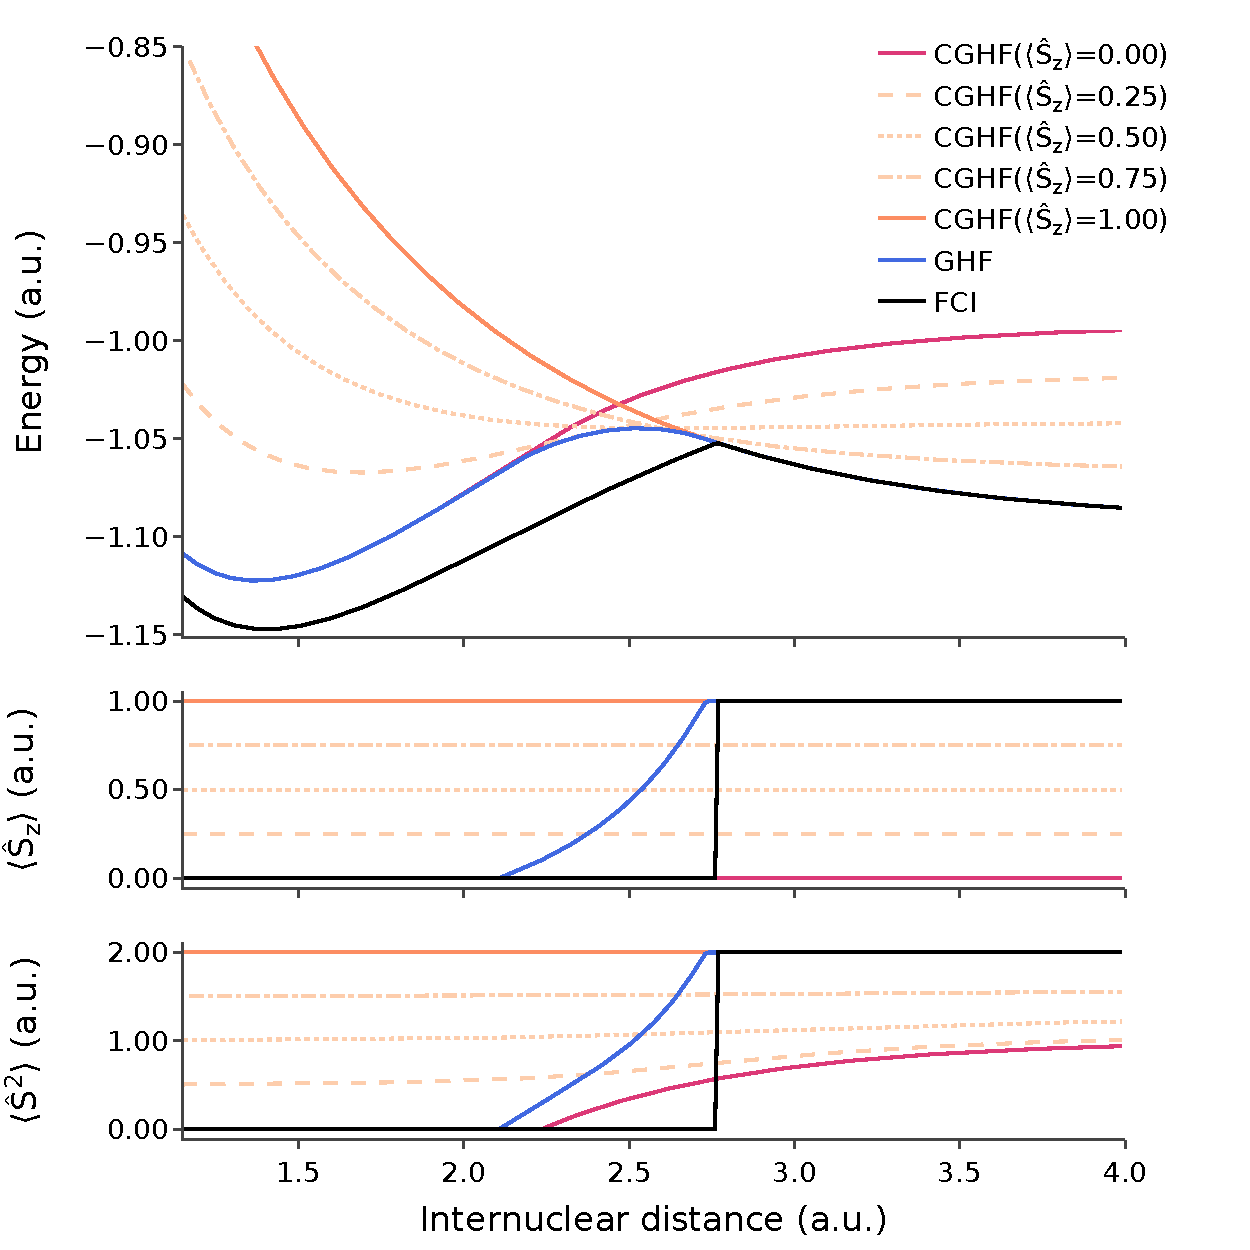
\includegraphics[width=0.65\textwidth]{C-GHF-PES(H2)(med-B)}
            \caption{
                (Unconstrained) GHF (blue), FCI (black) and Constrained GHF (CGHF, various colors) PES curves (top) and the corresponding spin expectation values ($\ev*{\hat{S}_z}$ (middle) and $\ev*{\hat{S}^2}$ (bottom)) for the dissociation of \ce{H2} in the presence of an external magnetic field $\vb{B}_{\text{ext}} = (0,0,-0.1)\text{ a.u}$.
                The spin expectation values $\ev*{\hat{S}_z}$ of the constrained GHF states are given between parentheses.
            }
            \label{fig:C-GHF-PES(H2)(med-B)}
        \end{figure}

        When \ce{H2} is stretched along the x-axis in the presence of an external magnetic field along the z-axis, FCI exhibits a discontinuous spin phase transition as two collinear states cross (see \cref{fig:C-GHF-PES(H2)(med-B)}).
        As GHF is able to break $\hat{S}_z$ symmetry, it is able to transition continuously both between the spin collinear (ordered) UHF$(M_S=0)$ phase and the spin non-collinear (disordered) phase as well as the spin non-collinear phase and the spin collinear UHF$(M_S=1)$ phase. 

        In the spin non-collinear phase, the respective CGHF potential energy surfaces (PES) are tangent to the GHF PES when their constraints are equal to the expected GHF spin projection $\ev*{\hat{S}_z}$. 
        The constrained states cross in the non-collinear spin phase as states with higher average projected spin become more stable than states with lower average projected spin. 
        At increasing bond lengths, GHF states constrained to low $\ev*{\hat{S}_z}$ rapidly spin contaminate, while states constrained to high $\ev*{\hat{S}_z}$ exhibit the same degree of spin contamination across the entire dissociation profile.

        \begin{figure}
            \centering
            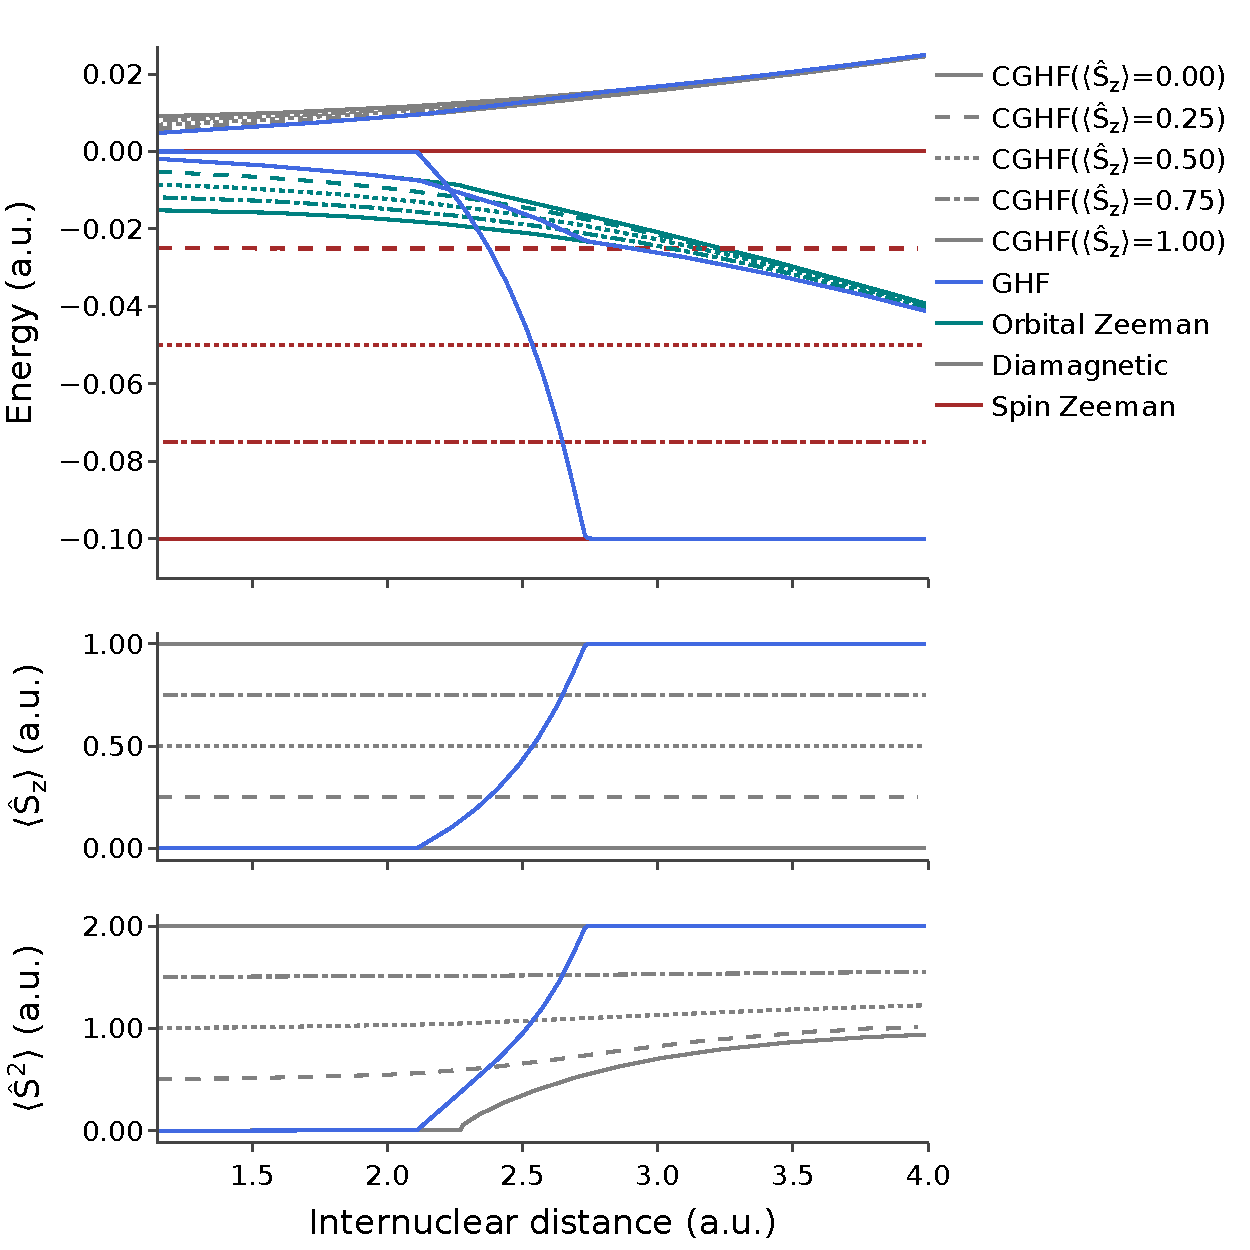
\includegraphics[width=0.65\textwidth]{C-GHF-energy-contributions(H2)(med-B)-S2}
            \caption{
                Orbital Zeeman (green), diamagnetic (gray) and spin Zeeman (red) energy contributions of the unconstrained GHF state (blue) and various constrained GHF states (dotted patterns) and the corresponding spin expectation values ($\ev*{\hat{S}_z}$ (middle) and $\ev*{\hat{S}^2}$ (bottom)) for the dissociation of \ce{H2} in an external magnetic field $\vb{B}_{\text{ext}} = (0,0,-0.1)\text{ a.u}$.
            }
            \label{fig:C-GHF-energy-contributions(H2)(med-B)}
        \end{figure}

        As the obtained CGHF states are well-behaved single Slater determinants we can compare their field-dependent energetic (i.e. orbital Zeeman, diamagnetic and spin Zeeman) contributions \cite{Sun.2019} (see \cref{fig:C-GHF-energy-contributions(H2)(med-B)}). 
        By breaking $S_z$ symmetry in the spin non-collinear phase, the GHF state is able to adequately balance decreasing exchange coupling with orbital Zeeman, diamagnetic and spin Zeeman contributions.
        At equilibrium, strong exchange coupling determines the spin behavior of the system, leading to a net destabilization of the energy with respect to the field-free case, as the positive energetic contributions of the diamagnetic term outweigh the stabilizing effects of the orbital Zeeman term \cite{Sun.2019}. By stretching the system, the reduction of the exchange coupling eventually leads to a phase transition into the non-collinear phase, where a non-zero $\ev*{\hat{S}_z}$ stabilizes the system through the spin Zeeman term. 
        
        For the CGHF state constrained to $\ev*{\hat{S}_z} = 0.0$, no such spin Zeeman stabilization can occur. As such, the orbital Zeeman and diamagnetic terms continue to determine the spin behavior by perturbing the spatial extent and energetics of the molecular orbitals \cite{Tellgren.2014, Sun.2019}. This leads to a discontinuity in the orbital Zeeman contribution at the position where the CGHF$(\ev*{\hat{S}_z}=0)$ state becomes spin contaminated (see \cref{fig:C-GHF-PES(H2)(med-B)}). On the other hand, the CGHF state constrained to $\ev*{\hat{S}_z} = 1.0$ is stabilized by spin Zeeman terms, which, however, leads to unfavorable exchange couplings at small internuclear distances (see \cref{fig:C-GHF-PES(H2)(med-B)}). At larger internuclear distance, these exchange couplings are reduced to the point where the spin Zeeman term determines the spin behavior and the spin collinear $M_S=1$ phase is favored.

        These results indicate that the constrained framework augments the electronic characterization of spin phases as it allows exploring the intricately balanced energetic competition between Coulombic and magnetic potentials by contrasting the behavior of the unconstrained minimum with those states that are fixed to a certain spin during dissociation. This allows one to unravel the interplay between the orbital Zeeman, diamagnetic and spin Zeeman contributions of the magnetic field to the molecular system.  
    
    \subsection{Spin phase diagrams quantify where Löwdin's dilemma occurs for GHF in magnetic fields}

        \begin{figure}
            \centering
            \begin{subfigure}[h]{0.45\textwidth}
                \centering
                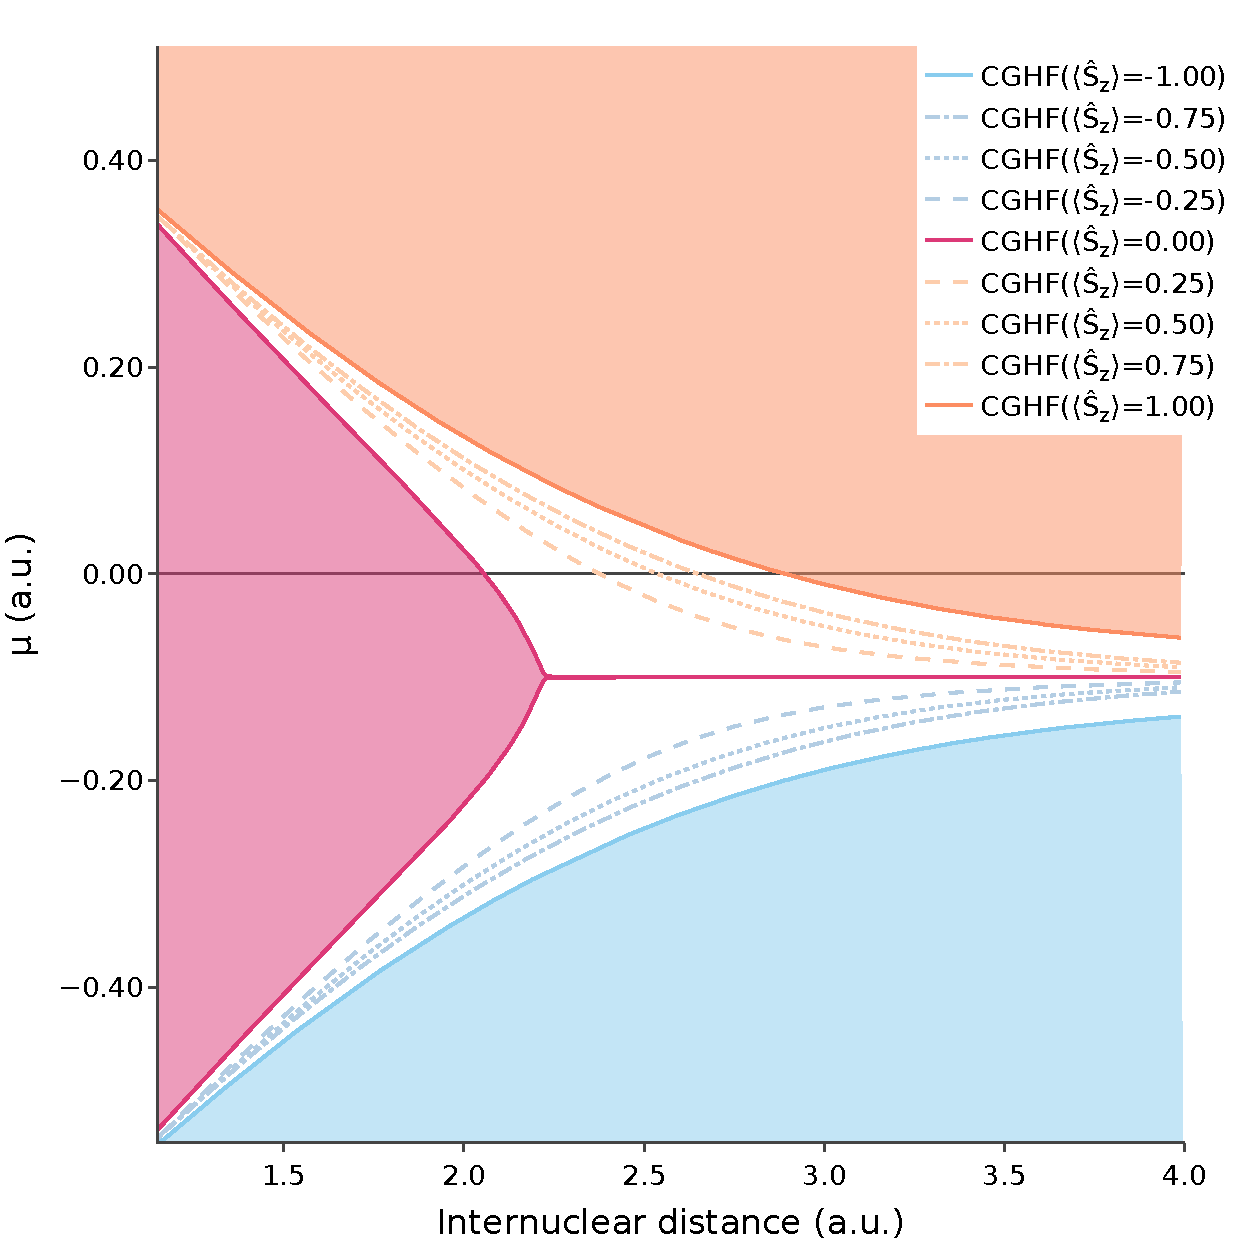
\includegraphics[width=\textwidth]{GHF-spin-phase-diagram(H2)(med-B)}
                \caption{CGHF}
                \label{fig:GHF-spin-phase-diagram-H2}
            \end{subfigure}
            \begin{subfigure}[]{0.45\textwidth}
                \centering
                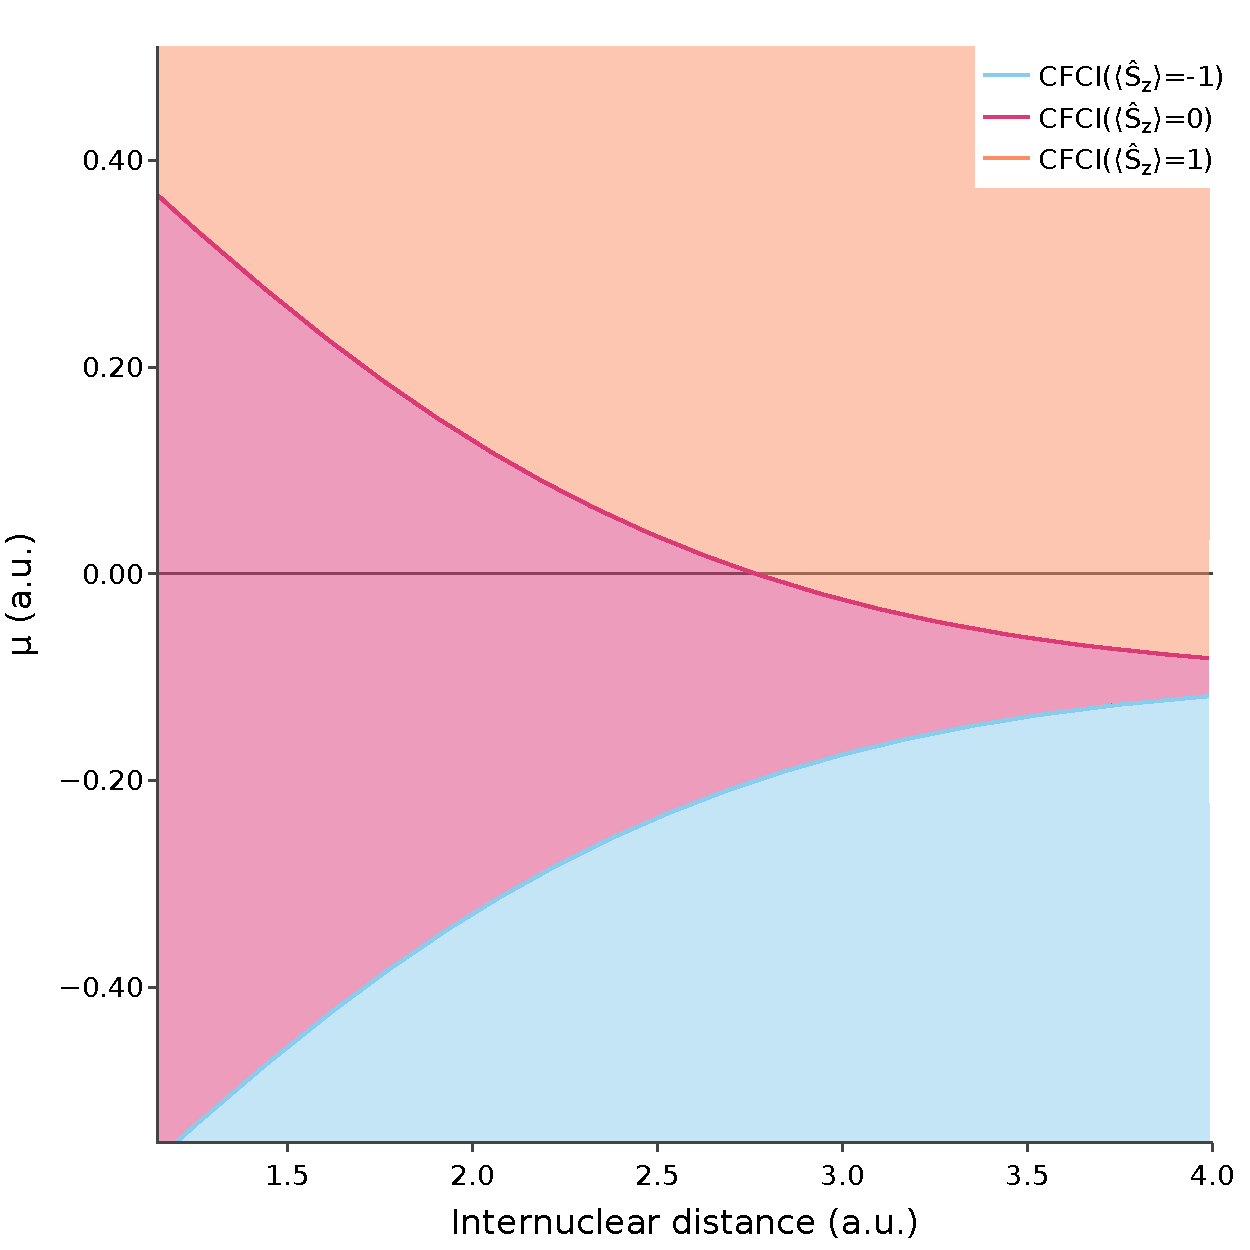
\includegraphics[width=\textwidth]{FCI-spin-phase-diagram(H2)(med-B)}
                \caption{FCI}
                \label{fig:FCI-spin-phase-diagram-H2}
            \end{subfigure}
            \caption{
                Spin phase diagram and selected states of \ce{H2} during its dissociation in the presence of an external magnetic field $\vb{B}_{\text{ext}} = (0,0,-0.1)\text{ a.u}$.
            }
            \label{fig:spin-phase-diagram-H2-med-B}
        \end{figure}

        By plotting the spin expectation value for the ground state as a function of the Lagrange multiplier $\mu_{S_z}$ and internuclear distance, we obtain the spin diagram associated with $\ce{H2}$ (see \cref{fig:spin-phase-diagram-H2-med-B}). 
        In these diagrams, the spin phases for the unconstrained case (see \cref{fig:C-GHF-PES(H2)(med-B)}) are situated along the $\mu=0$ horizontal line. 
        In contrast, as the Lagrange potential is proportional to the spin Zeeman term, a horizontal line at $\mu = - \abs{B_{\text{ext}, z}}$ corresponds to a system where explicit spin-magnetic field interactions are absent and thus only the orbital Zeeman and diamagnetic terms remain (see \cref{eq:Pauli-Hamiltonian}, \cref{eq:pauli-matrices} and \cref{eq:modified-Hamiltonian}).
        Therefore, a vertical line in a spin phase diagram corresponds to a tuning of the spin Zeeman term at a particular point during the dissociation process.
        By combining such horizontal and vertical movements, we can describe different \emph{trajectories} through the spin phase diagram, allowing us to explore different spin phases and the transitions that exist between them.

        In the case of FCI (see \cref{fig:FCI-spin-phase-diagram-H2}), there are three collinear spin phases, associated with $M_S=-1$, $M_S=0$ and $M_S=-1$ indicated by orange, red and blue regions, respectively.
        The transitions between these phases are discontinuous, leading to discontinuous potential energy surfaces and spin surfaces (see \cref{fig:C-GHF-PES(H2)(med-B)}). 
        In the case of GHF, there exists an additional non-collinear/disordered phase, in which GHF breaks $S_z$-symmetry. 
        This disordered phase quantifies where Löwdin's dilemma matters and offers a unique perspective on the physics of the intermediate coupling regime as it straddles the limiting cases of collinear spin phases \cite{sachdev2011a}.
        We note that, as the CGHF states effectively span the entire disordered phase, they could provide an excellent starting point for post-Hartree Fock methods aimed at gaining more electron correlation or regaining spin symmetry \cite{Thom.2009, Sundstrom.2014, Burton.2021}.

    \subsection{Characterizing the influence of the magnetic field with spin phase diagrams}
        
        \begin{figure}
            \centering
            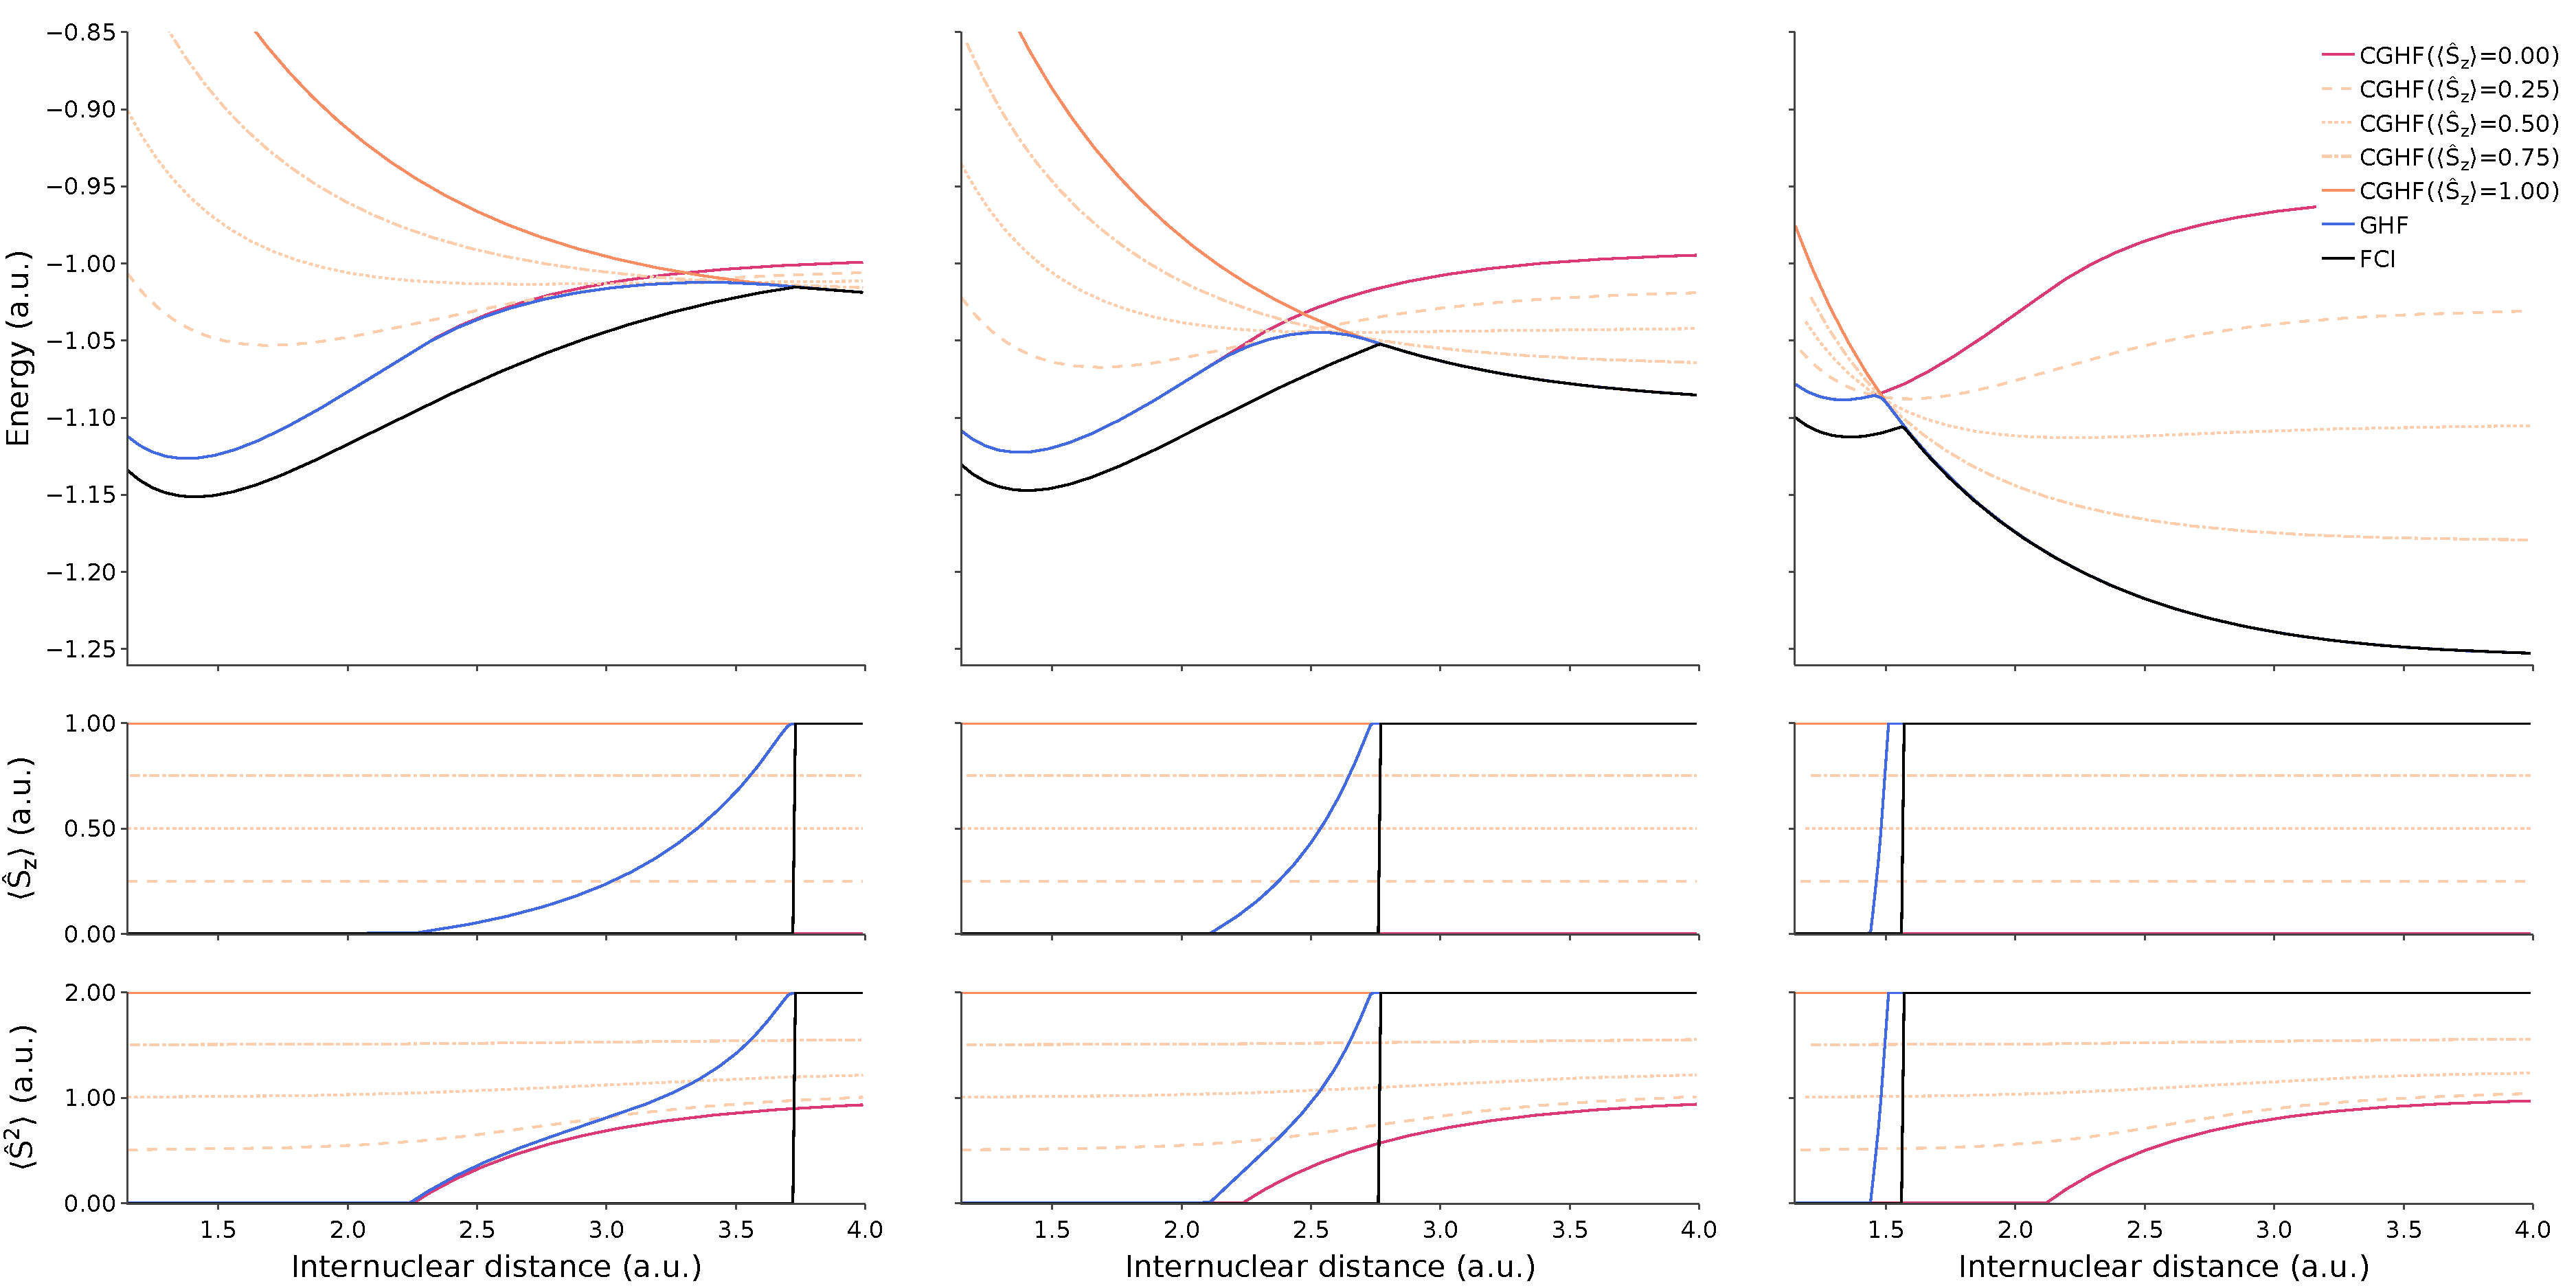
\includegraphics[width=\textwidth]{C-GHF-PES(H2)-S2}
            \caption{
                Unconstrained GHF (blue), FCI (black) and constrained GHF (CGHF, various colors) PES curves (top) and the corresponding spin expectation value $\ev*{\hat{S}_z}$ (bottom) for the dissociation of \ce{H2} in different external magnetic fields.
                Left, $\vb{B}_{\text{ext}} = (0,0,-0.03)\text{ a.u}$.
                Middle, $\vb{B}_{\text{ext}} = (0,0,-0.1)\text{ a.u}$.
                Right, $\vb{B}_{\text{ext}} = (0,0,-0.3)\text{ a.u}$.
            }
            \label{fig:C-GHF-PES(H2)}
        \end{figure}
        
        Increasing the strength of the magnetic field $\vb{B}_{\text{ext}}$ leads to smaller ranges of internuclear distance where CGHF states cross, which is echoed by rapidly increasing $\ev*{\hat{S}_z}$ in the non-collinear phase as a function of internuclear distance (see \cref{fig:C-GHF-PES(H2)}).
        At small internuclear distances, the energies of the GHF and FCI states rise with increasing field strength and the CGHF states become more tightly bundled in a narrower energy range.
        At large internuclear distances, the GHF and FCI states drop significantly in energy with increasing field strength. 
        In contrast, the entire PES of the CGHF($\ev*{\hat{S}_z}=0.0$) rises in energy with increasing field strength, while all other CGHF are lowered, with greater energy lowerings for states constrained to higher $\ev*{\hat{S}_z}$.
        
        \begin{figure}
            \centering
            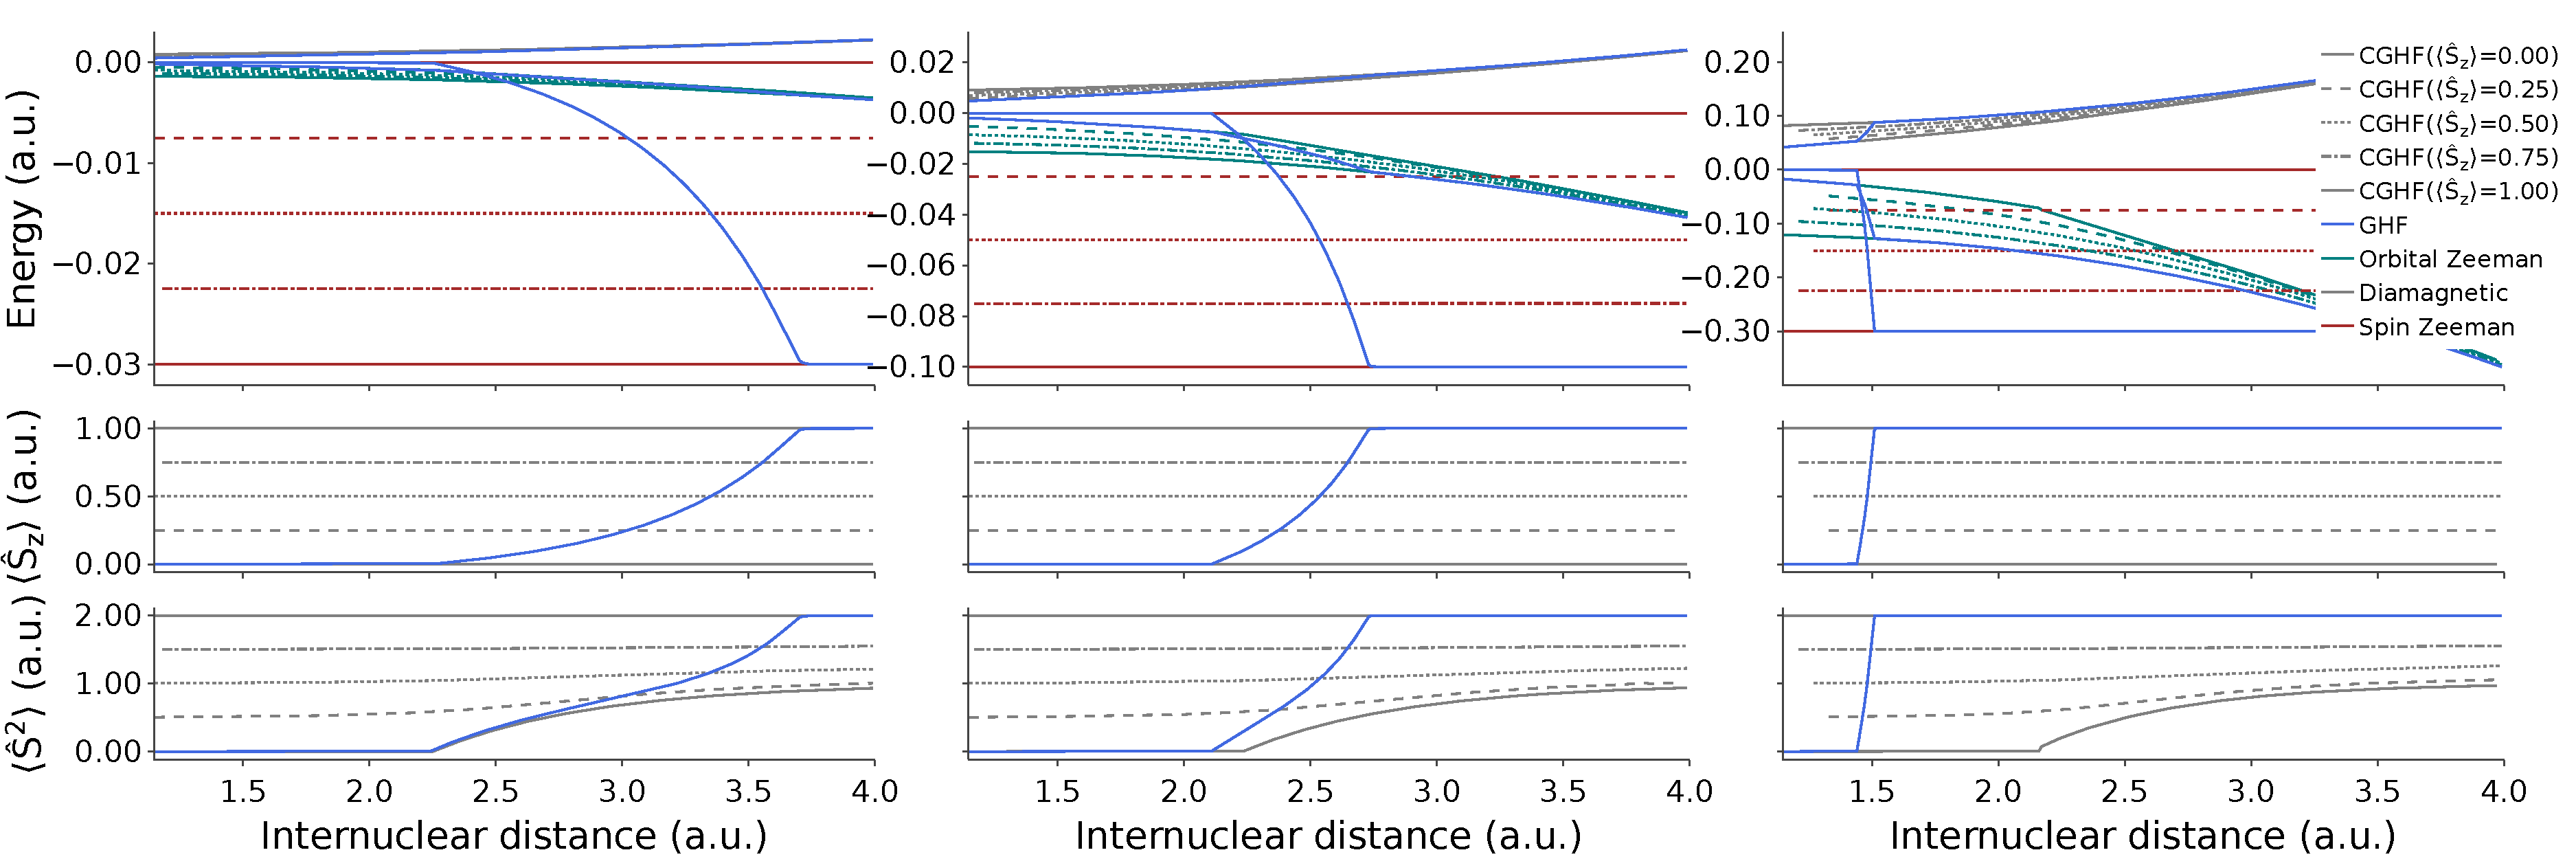
\includegraphics[width=\textwidth]{C-GHF-energy-contributions(H2)}
            \caption{
                Orbital Zeeman (green), diamagnetic (gray) and spin Zeeman (red) energy contributions of the unconstrained GHF (blue) state and various constrained GHF-states during the dissociation of \ce{H2} in different external magnetic fields.
                Left, $\vb{B}_{\text{ext}} = (0,0,-0.03)\text{ a.u}$.
                Middle, $\vb{B}_{\text{ext}} = (0,0,-0.1)\text{ a.u}$.
                Right, $\vb{B}_{\text{ext}} = (0,0,-0.3)\text{ a.u}$.
            }
            \label{fig:C-GHF-energy-contributions(H2)}
        \end{figure}

        The different orbital Zeeman, diamagnetic and spin Zeeman contributions for the respective magnetic fields (see \cref{fig:C-GHF-energy-contributions(H2)}) show that the three GHF spin phases are each characterized by a different behavior. 
        In the collinear $\ev*{\hat{S}_z}=0.0$ phase, increasing diamagnetic energy contributions determine the increase in GHF energy with increasing field strength. 
        In the non-collinear phase, the GHF energy drops paramagnetically, due to the relaxation associated with the spin Zeeman stabilization of the broken spin symmetry state.
        In the collinear $\ev*{\hat{S}_z}=1.0$ phase, the GHF energy drops paramagnetically with increasing magnetic field predominantly due to orbital Zeeman contributions.
        
        The quadratic scaling behavior of the orbital Zeeman term with increasing magnetic field can be related to the paramagnetic bonding mechanism introduced by Helgaker et al \cite{Lange.2012}. 
        In this mechanism, the kinetic energy is lowered due to an induced paramagnetic rotation of the s-orbitals to p-orbitals oriented along the magnetic field, which couple linearly to the magnetic field. 
        As such, the diamagnetic and orbital Zeeman indirectly influence the spin behavior by perturbing the molecular orbitals, as also shown by the onset of spin contamination in the CGHF($\ev*{\hat{S}_z}=0.0$) state, which is marked by a discontinuity in the orbital Zeeman contribution. 

        \begin{figure}
            \centering
            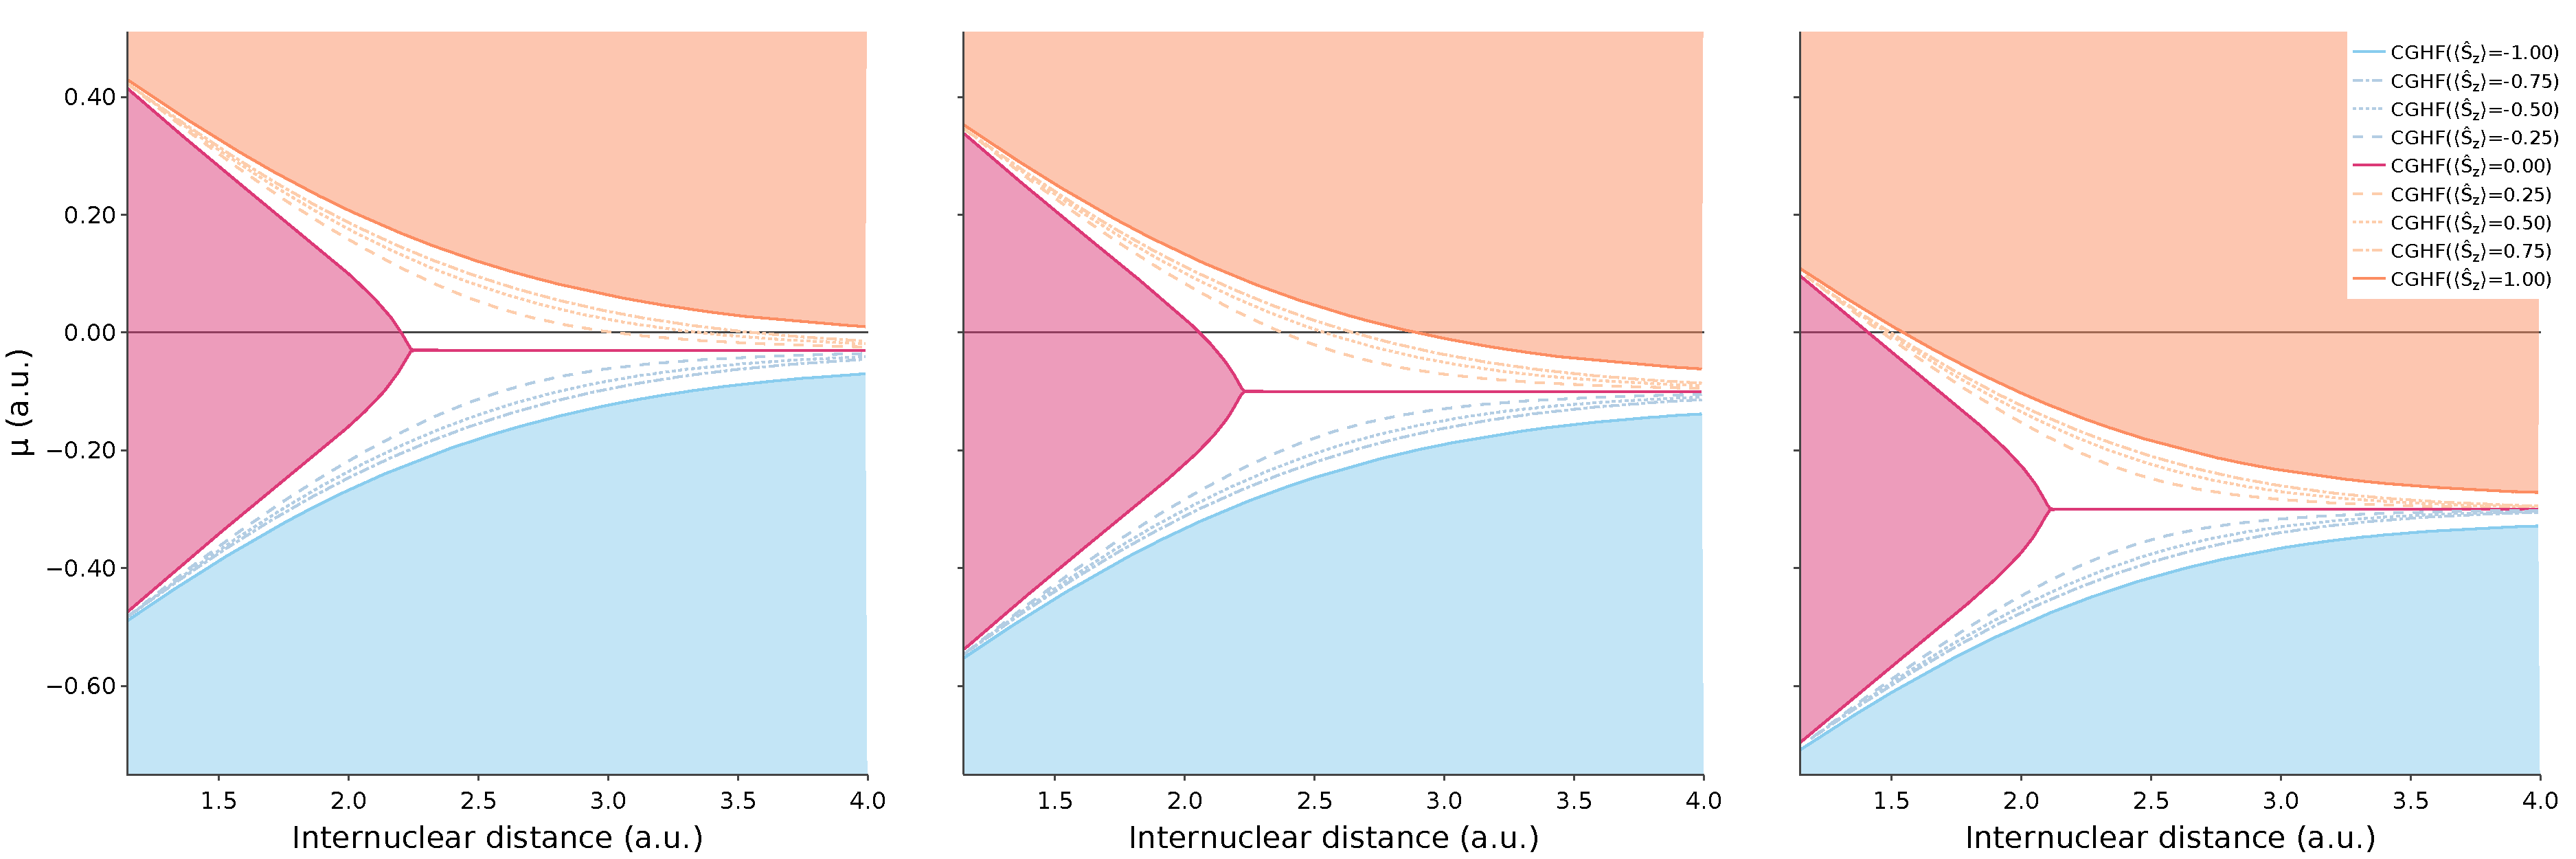
\includegraphics[width=\textwidth]{GHF-spin-phase-diagram(H2)}
            \caption{
                GHF spin phase diagram and selected CGHF states (dashed) of \ce{H2} during its dissociation in different external magnetic fields.
                Left, $\vb{B}_{\text{ext}} = (0,0,-0.03)\text{ a.u}$.
                Middle, $\vb{B}_{\text{ext}} = (0,0,-0.1)\text{ a.u}$.
                Right, $\vb{B}_{\text{ext}} = (0,0,-0.3)\text{ a.u}$.
            }
            \label{fig:GHF-spin-phase-diagram(H2)}
        \end{figure}

        % \begin{figure}
        %     \centering
        %     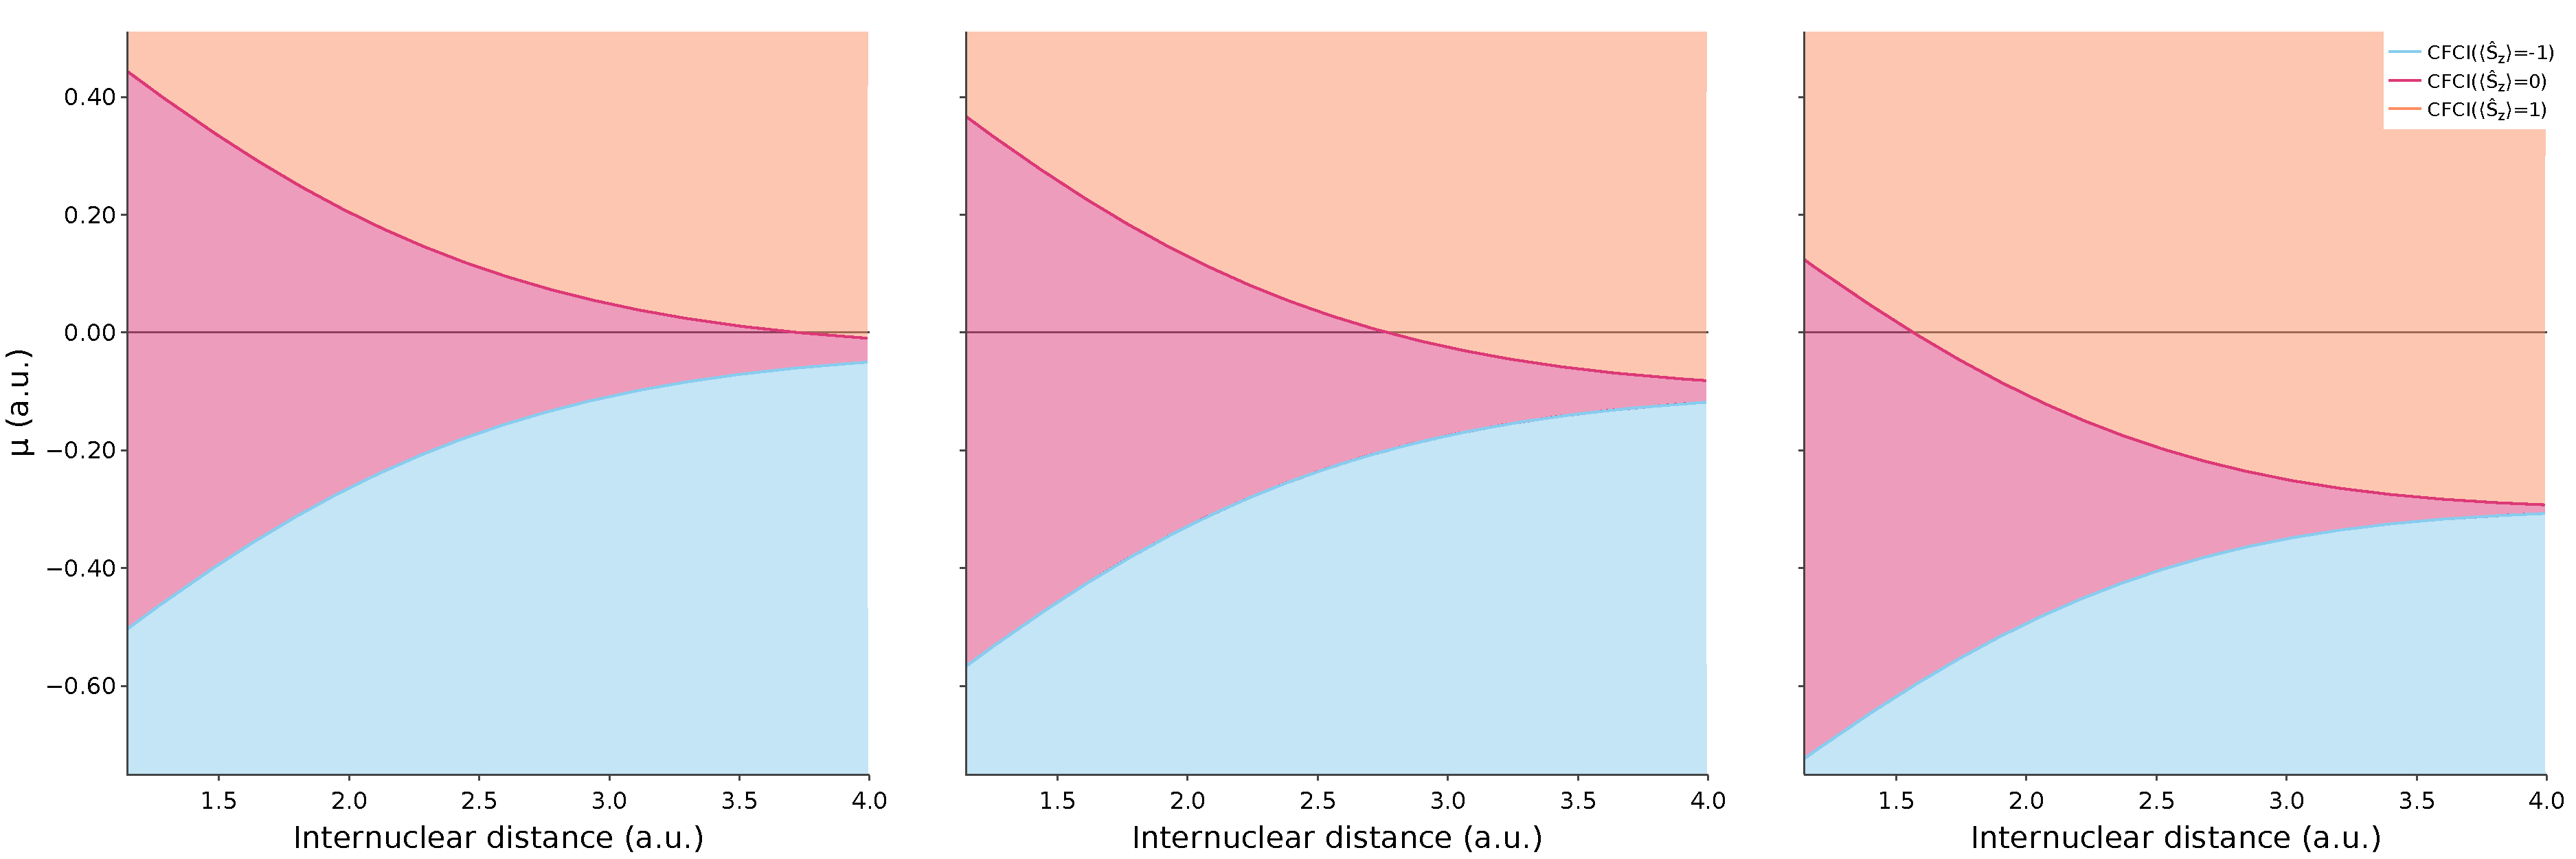
\includegraphics[width=\textwidth]{FCI-spin-phase-diagram(H2)}
        %     \caption{
        %         FCI spin phase diagram (top) and spin expectation value $\ev*{\hat{S}_z}$ (bottom) of \ce{H2} during its dissociation in different external magnetic fields.
        %         Left, $\vb{B}_{\text{ext}} = (0,0,-0.03)\text{ a.u}$.
        %         Middle, $\vb{B}_{\text{ext}} = (0,0,-0.1)\text{ a.u}$.
        %         Right, $\vb{B}_{\text{ext}} = (0,0,-0.3)\text{ a.u}$.
        %     }
        %     \label{fig:FCI-spin-phase-diagram(H2)}
        % \end{figure}

        The associated spin phase diagrams provide more insight into this discontinuity in the orbital Zeeman contribution (see \cref{fig:GHF-spin-phase-diagram(H2)}). 
        With increasing magnetic field, larger negative potentials $\mu = - \abs{B_{\text{ext}, z}}$ are required to negate the effects of the spin Zeeman term, effectively pushing the spin diagrams down. 
        Combined with orbital Zeeman and diamagnetic contributions, this increasing magnetic field also enlarges the high spin phases, effectively compressing the non-collinear and $M_S=0$ phases.
        As such, the horizontal $\mu=0$ line cuts smaller regions of the non-collinear spin phase, leading to more steeply increasing $\ev*{\hat{S}_z}$.
        If we constrain the GHF state to $\ev*{\hat{S}_z}=0$ phase, then, with increasing internuclear distance, the state initially remains in the spin collinear phase and move along the edge of this phase towards the pointed tip.
        With even larger internuclear distance, this constrained GHF state is forced to transition into the non-collinear phase with a concomitant spin contamination.

    \subsection{Characterizing spin behavior in \ce{H4}-rings with spin diagrams}

        \begin{figure}
            \centering
            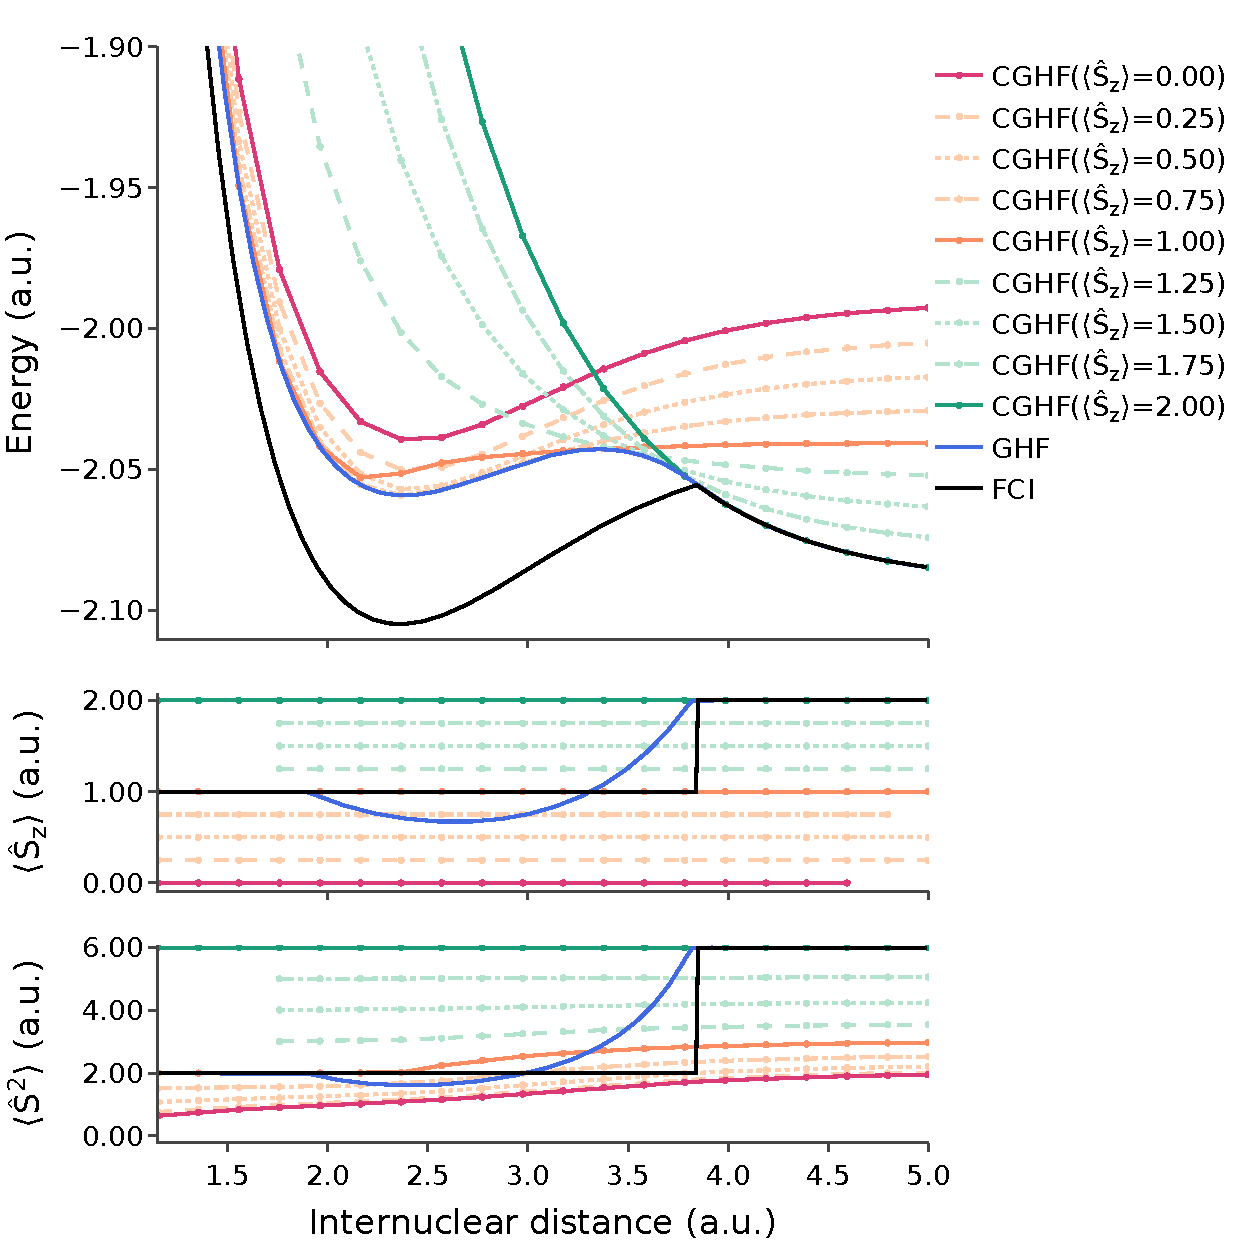
\includegraphics[width=0.65\textwidth]{C-GHF-PES(H4)(med-B)}
            \caption{
                Unconstrained GHF (blue), FCI (black) and constrained GHF (CGHF, various colors) PES curves (top) and the corresponding spin expectation values $\ev*{\hat{S}_z}$ (middle) and $\ev*{\hat{S}^2}$ (bottom) for the dissociation of equilateral cyclic \ce{H4} in an external magnetic field $\vb{B}_{\text{ext}} = (0,0,-0.05)\text{ a.u}$.
                Points for which the constraint could not be met are not plotted. Internuclear distance corresponds to the distance between two adjacent hydrogen atoms in the \ce{H4} square.                 
            }
            \label{fig:C-GHF-PES(H4)(med-B)}
        \end{figure}   

        We next study the symmetric dissociation of equilateral cyclic \ce{H4} in the presence of an external magnetic field $\vb{B}_{\text{ext}} = (0,0,-0.05)\text{ a.u.}$ oriented orthogonal to the molecular plane. In stark contrast to the spin behavior of GHF in molecular hydrogen, GHF exhibits at first a \emph{decrease} in $\ev*{\hat{S}_z}$ during the symmetric dissociation (see \cref{fig:C-GHF-PES(H4)(med-B)}). 
        Only after reaching a minimum $\ev*{\hat{S}_z}$ does the expected spin projection increase uniformly towards $\ev*{\hat{S}_z} = 2$.
        The CGHF states with $\ev*{\hat{S}_z} \geq 1.25$ exhibit a uniformly lowering energy as a function of the internuclear distance, while CGHF states with $\ev*{\hat{S}_z} \leq 1.0$ have bound minima around 2.5 a.u.
        The latter states show high amounts of spin contamination, where the onset of spin contamination for the CGHF($\ev*{\hat{S}_z}=1.0$) state starts around 2.4 a.u., pointing at significant magnetically induced orbital rotations.
        The resulting spin behavior for the CGHF($\ev*{\hat{S}_z}=1.0$) state  cause the associated PES to deviate from the PES associated with states constrained to $\ev*{\hat{S}_z} < 1.0$.
        
        \begin{figure}
            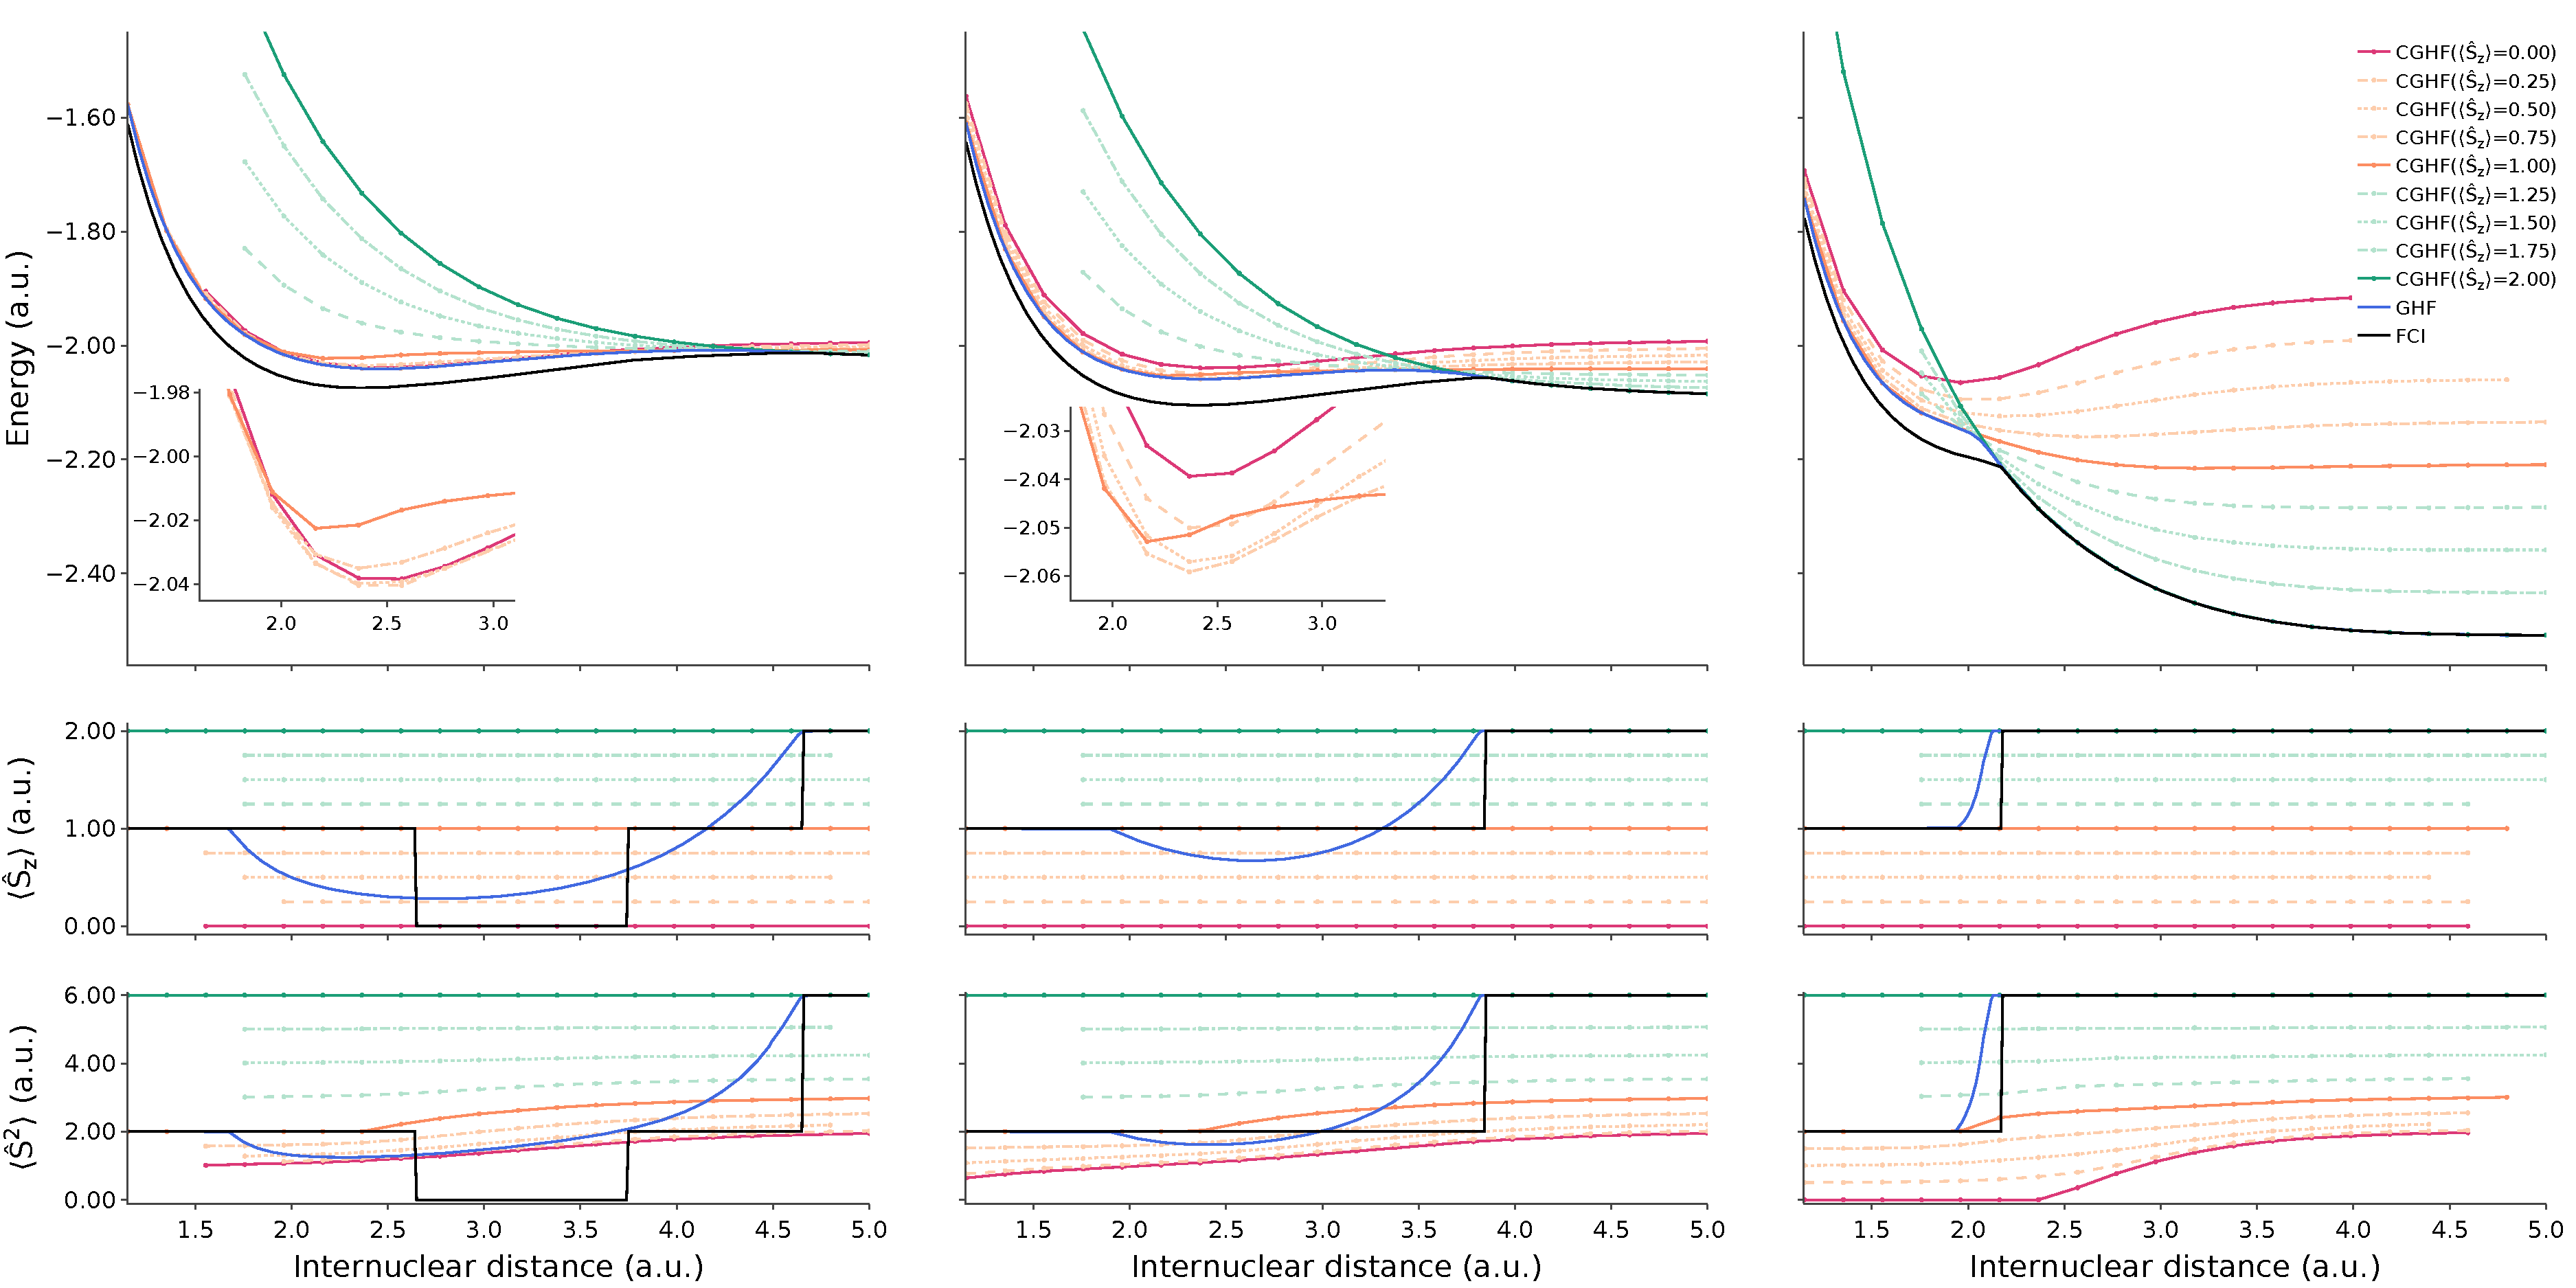
\includegraphics[width=\textwidth]{C-GHF-PES(H4)}
            \caption{
                Unconstrained GHF (blue), FCI (black) and constrained GHF (CGHF, various colors) PES curves (top) and the corresponding spin expectation values $\ev*{\hat{S}_z}$ (middle) and $\ev*{\hat{S}^2}$ (bottom) for the dissociation of equilateral cyclic \ce{H4} in different external magnetic fields.
                Points for which the constraint could not be met are not plotted.    
                Left: $\vb{B}_{\text{ext}} = (0,0,-0.015)\text{ a.u}$.
                Middle: $\vb{B}_{\text{ext}} = (0,0,-0.05)\text{ a.u}$.
                Right: $\vb{B}_{\text{ext}} = (0,0,-0.3)\text{ a.u}$.
            }
            \label{fig:C-GHF-PES(H4)}
        \end{figure}

        By tuning the magnetic field, we gain more insight into the chemical reasons behind the spin behavior at $\vb{B}_{\text{ext}} = (0,0,-0.05)\text{ a.u.}$ (see \cref{fig:C-GHF-PES(H4)}). 
        At lower magnetic fields, the lowest expected spin projection $\ev*{\hat{S}_z}$ drops to 0.25, and, at intermediate bonding distance, FCI drops to a lower spin symmetry sector.
        Whereas the potential energy surfaces associated with CGHF($\ev*{\hat{S}_z} \geq 1.0$) remain essentially unchanged, the CGHF($\ev*{\hat{S}_z} <  1.0$) states drop below the CGHF($\ev*{\hat{S}_z}=1.0$) state in the bonding region.
        As such, in the bonding region at low magnetic fields, the chemistry of the system is influenced by the exchange coupling in the hydrogen ring, striving towards the net zero expected value of $\hat{S}_z$ and spin contamination slightly larger than one that is characteristic of broken symmetry solutions for \ce{H4} \cite{Goings.2015}.

        At higher magnetic fields, the CGHF($\ev*{\hat{S}_z}=0$) state is no longer spin contaminated at low internuclear distances and is a pure $M_S=0$ phase, indicating that the spin behavior of \ce{H4} essentially correspond to two \ce{H2} molecules.
        Furthermore, the average GHF spin projection never drops below 1.0 while spin contamination rises rapidly, indicating a high degree of spin frustration.

        \begin{figure}
            \centering
            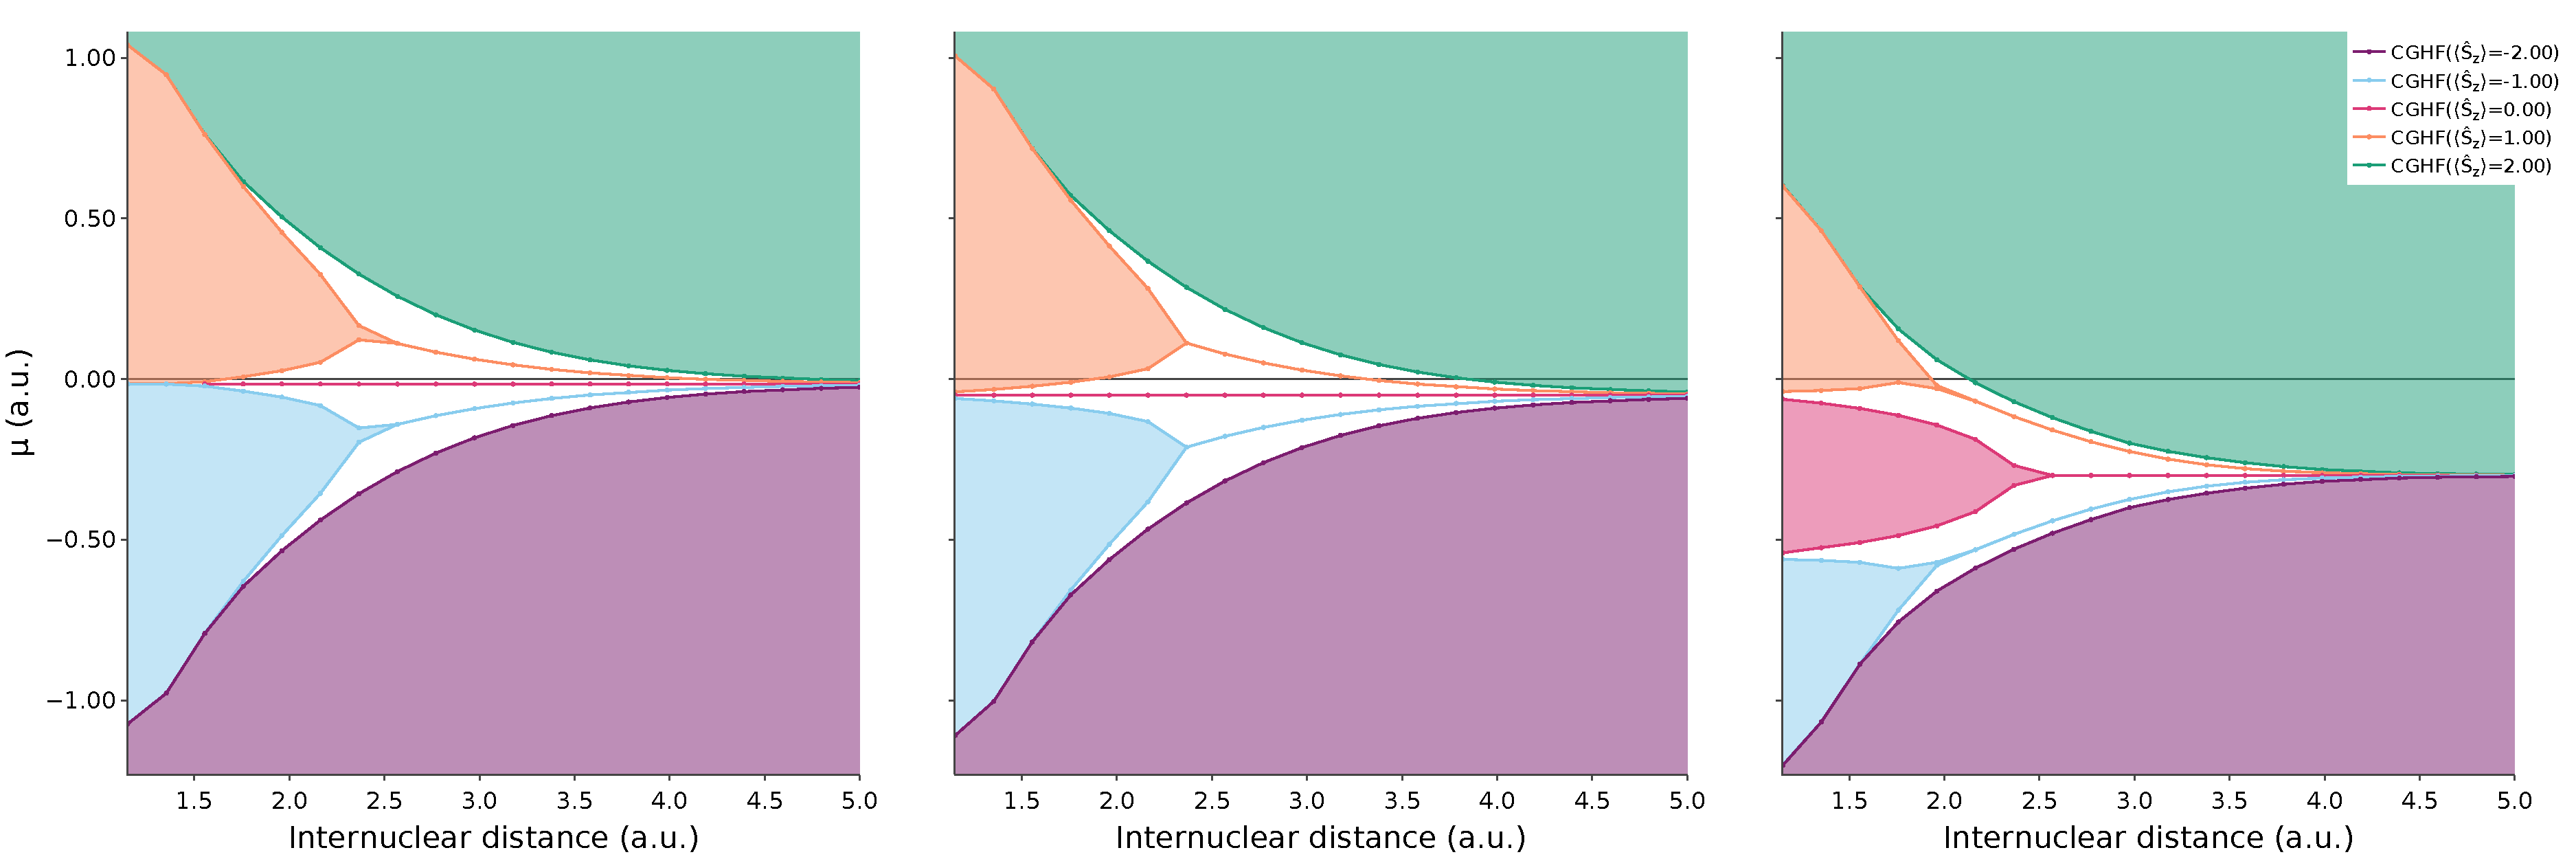
\includegraphics[width=\textwidth]{GHF-spin-phase-diagram(H4)}
            \caption{
                GHF spin phase diagrams (top) and the corresponding spin expectation value $\ev*{\hat{S}_z}$ (bottom) for the dissociation of equilateral cyclic \ce{H4} in the presence of different external magnetic fields.
                Left: $\vb{B}_{\text{ext}} = (0,0,-0.015)\text{ a.u}$.
                Middle: $\vb{B}_{\text{ext}} = (0,0,-0.05)\text{ a.u}$.
                Right: $\vb{B}_{\text{ext}} = (0,0,-0.3)\text{ a.u}$.
            }
            \label{fig:GHF-spin-phase-diagram-H4}
        \end{figure}

        % \begin{figure}
        %     \centering
        %     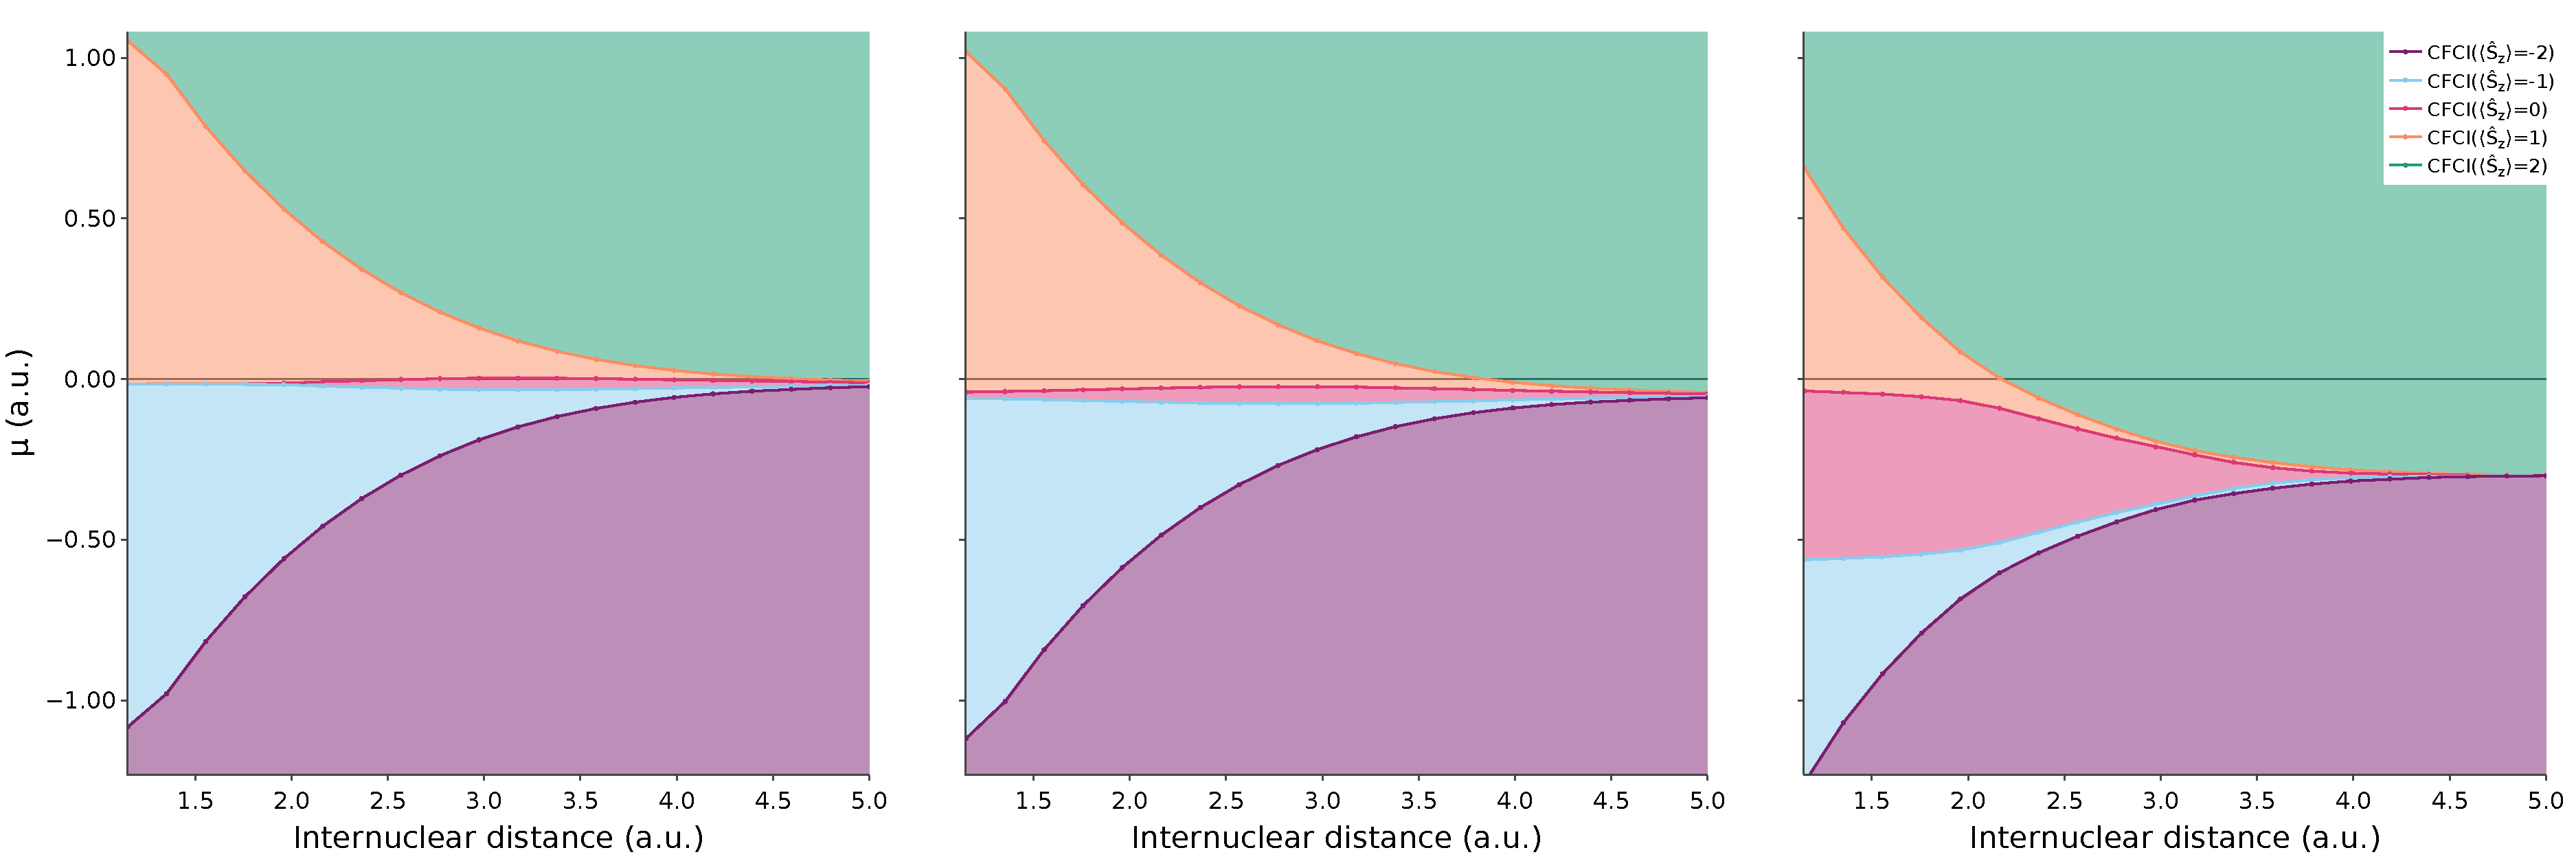
\includegraphics[width=\textwidth]{FCI-spin-phase-diagram(H4)}
        %     \caption{
        %         FCI spin phase diagrams (top) and the corresponding spin expectation value $\ev*{\hat{S}_z}$ (bottom) for the dissociation of equilateral cyclic \ce{H4} in the presence of different external magnetic fields.
        %         Left: $\vb{B}_{\text{ext}} = (0,0,-0.015)\text{ a.u}$.
        %         Middle: $\vb{B}_{\text{ext}} = (0,0,-0.05)\text{ a.u}$.
        %         Right: $\vb{B}_{\text{ext}} = (0,0,-0.3)\text{ a.u}$.
        %     }
        %     \label{fig:FCI-spin-phase-diagram-H4}
        % \end{figure}

        This viewpoint is reinforced by the spin phase diagram (see \cref{fig:GHF-spin-phase-diagram-H4}). With increasing magnetic field, the corresponding GHF phase diagram gains an additional collinear phase with $M_S=0$ (see \cref{fig:GHF-spin-phase-diagram-H4}) associated with the spin behavior of two hydrogen molecules.
        At low magnetic field, unconstrained GHF (i.e. $\mu=0$) tries to accommodate as much of the changing exchange forces as possible in the non-collinear phase, actively breaking $\hat{S}_z$ symmetry to come as close as possible to the field-free UHF $M_S=0$ description.
        At intermediate magnetic fields, the spin behavior straddles between both extremes, leading to $\ev*{\hat{S}_z}$ behavior that at first might seem unexpected.
        
        As such, these results show that GHF is able to resound the echoes of its field-free behavior into its description of the influence of a magnetic field. Consequently, the breaking of symmetries not only leads to continuous transitions in potential energy surfaces, but also leads to continuous transitions in the description of increasing magnetic fields.

\section{Conclusions}
    In this study, we have shown that the constrained framework augments the electronic characterization of spin phases as it allows to contrast the behavior of the unconstrained minimum with those states that are fixed to a certain spin. To that end, an additional term was added to the Hamiltonian to impose a desired expectation value for $\hat{S}_z$.
    By unravelling the interplay between the orbital Zeeman, diamagnetic and spin Zeeman contributions when applying a magnetic field to a molecular system, we could elucidate how such a uniform magnetic field influences the energetics and spin behavior of \ce{H2} and equilateral cyclic \ce{H4} during dissociation.
    As the constrained GHF states effectively span the entire phase space, they could provide an excellent starting point for post-Hartree Fock methods aimed at gaining more electron correlation or regaining spin symmetry.

\section*{Authors' contributions}
    L.L. was the project, software and visualization lead; he equally conceived the project, wrote the original draft and equally contributed in editing the draft.
    X.D.V. supported the software development and visualization.
    P.B. is the funding acquisition lead; he reviewed the manuscript and contributed in editing.
    G.A. was the review and editing lead and equally conceived the project; he contributed to the original draft and equally contributed in the funding acquisition.



%%%%%%%%%%%%%%%%%%%%%%%%%%%%%%%%%%%%%%%%%%%%%%%%%%%%%%%%%%%%%%%%%%%%%
%% The "Acknowledgement" section can be given in all manuscript
%% classes.  This should be given within the "acknowledgement"
%% environment, which will make the correct section or running title.
%%%%%%%%%%%%%%%%%%%%%%%%%%%%%%%%%%%%%%%%%%%%%%%%%%%%%%%%%%%%%%%%%%%%%
\begin{acknowledgement}
    L.L. acknowledges support from an FWO Ph.D. fellowship (Grant No. 1126619N).
    Parts of this research were also funded by the FWO (Research Project No. G031820N).
    The computational resources (Stevin Supercomputer Infrastructure) and services used in this work were provided by the VSC (Flemish Supercomputer Center), funded by Ghent University, FWO and the Flemish Government - department EWI.
\end{acknowledgement}


%%%%%%%%%%%%%%%%%%%%%%%%%%%%%%%%%%%%%%%%%%%%%%%%%%%%%%%%%%%%%%%%%%%%%
%% The same is true for Supporting Information, which should use the
%% suppinfo environment.
%%%%%%%%%%%%%%%%%%%%%%%%%%%%%%%%%%%%%%%%%%%%%%%%%%%%%%%%%%%%%%%%%%%%%
\section*{Data availability}
    The data and software that support the findings of this study are available on \url{https://github.com/GQCG-res/spin-diagrams}.


%%%%%%%%%%%%%%%%%%%%%%%%%%%%%%%%%%%%%%%%%%%%%%%%%%%%%%%%%%%%%%%%%%%%%
%% The appropriate \bibliography command should be placed here.
%% Notice that the class file automatically sets \bibliographystyle
%% and also names the section correctly.
%%%%%%%%%%%%%%%%%%%%%%%%%%%%%%%%%%%%%%%%%%%%%%%%%%%%%%%%%%%%%%%%%%%%%
\bibliography{paper}

\end{document}
